% chapters/05 - chapter5.tex
\chapter{Phép tính tích phân}

Từ thời cổ đại, con người đã phát triển các ý niệm trực quan về độ dài, diện tích và thể tích để đáp ứng nhu cầu đo lường trong cuộc sống. Tuy nhiên, việc định nghĩa một cách chặt chẽ và tổng quát cho các khái niệm này, đặc biệt là diện tích của những hình có biên cong, lại là một thách thức lớn của toán học. Chúng ta quen thuộc với việc tính diện tích các hình đơn giản như hình chữ nhật, hình tam giác, hay bất kỳ đa giác nào bằng cách chia nó thành các tam giác nhỏ hơn. Nhu cầu xác định diện tích của những miền cong phức tạp hơn đã thúc đẩy sự ra đời của một công cụ toán học mạnh mẽ và tổng quát, đó chính là phép tính tích phân. Trong chương này, chúng ta sẽ khám phá cách xây dựng khái niệm tích phân một cách có hệ thống, bắt đầu từ phương pháp của Riemann.

\section{Định nghĩa và tính chất của tích phân}

Các khái niệm quen thuộc như độ dài, diện tích, và thể tích đã xuất hiện từ rất sớm trong lịch sử loài người, gắn liền với nhu cầu thực tiễn về đo lường. Mặc dù chúng ta có thể hình dung một cách trực quan rằng đây là những ``số đo'' về kích thước hay ``độ lớn'' của một vật thể, việc đưa ra một định nghĩa toán học chặt chẽ cho chúng không hề đơn giản, đặc biệt là câu hỏi: ``Làm thế nào để định nghĩa diện tích một cách tổng quát?''

Đối với những hình học cơ bản, câu trả lời có vẻ dễ dàng. Diện tích của một hình chữ nhật được xác định bằng tích chiều dài và chiều rộng. Từ đó, ta có thể suy ra công thức cho diện tích tam giác, và xa hơn là bất kỳ đa giác nào bằng cách phân chia nó thành các tam giác nhỏ. Tuy nhiên, phương pháp này trở nên bất lực trước những hình có đường biên cong.

Về mặt lịch sử, việc sử dụng khái niệm diện tích trong thực tế thường dựa trên hai nguyên tắc cơ bản: 
\begin{enumerate}[label=(\arabic*)]
    \item Chọn một hình làm ``đơn vị'' đo.
    \item Diện tích có tính chất cộng tính, tức là diện tích của một hình ghép bằng tổng diện tích các hình thành phần.
\end{enumerate}
Cách tiếp cận này, tuy hữu ích, nhưng vẫn chưa đủ để giải quyết bài toán một cách tổng quát.

Phải đến thế kỷ 17, với sự phát triển của giải tích, nhu cầu về một phương pháp tổng quát và chính xác để định nghĩa và tính toán diện tích mới thực sự được giải quyết. Vấn đề này đã dẫn đến sự hình thành của một phép toán tổng quát hóa quá trình cộng, được gọi là \textbf{phép tính tích phân}. Dưới đây, chúng ta sẽ bắt đầu tìm hiểu một trong những cách tiếp cận nền tảng nhất để xây dựng khái niệm này, được biết đến với tên gọi \textbf{tích phân Riemann}.

\subsection{Định nghĩa tích phân}

Xét một hàm số $f$ không âm, $f: [a, b] \to \R$. Mục tiêu của chúng ta là xác định ``diện tích'' của miền phẳng giới hạn bởi đồ thị của hàm $f$, trục hoành, và hai đường thẳng đứng $x=a, x=b$. Ý tưởng cơ bản là xấp xỉ miền cong này bằng một tập hợp các hình chữ nhật đơn giản. Đáy của mỗi hình chữ nhật là một đoạn con của $[a,b]$ và chiều cao được xác định bởi một giá trị của hàm $f$ trên đoạn con đó. Ta kỳ vọng rằng, khi chúng ta sử dụng ngày càng nhiều hình chữ nhật (tức là làm cho các đáy ngày càng nhỏ), tổng diện tích của chúng sẽ tiến gần đến giá trị diện tích thực của miền đang xét (xem Hình \ref{fig:rectangle_approx}).

Ta có thể cụ thể hóa ý tưởng này như sau. Trước hết, ta thực hiện một phép phân hoạch đoạn $[a, b]$ bằng một dãy các điểm:
\[ a = x_0 < x_1 < x_2 < \dots < x_n = b. \]
Phép phân hoạch này chia đoạn $[a, b]$ thành $n$ đoạn con $[x_{i-1}, x_i]$, với $i = 1, 2, \dots, n$. Trên mỗi đoạn con $[x_{i-1}, x_i]$, ta chọn một điểm bất kỳ $x_i^*$ và gọi nó là \textit{điểm mẫu}. Giá trị $f(x_i^*)$ được xem là chiều cao đại diện cho đồ thị của hàm $f$ trên toàn bộ đoạn con đó. Khi đó, ta có thể xây dựng một hình chữ nhật với đáy là $[x_{i-1}, x_i]$ (có độ dài là $\Delta x_i = x_i - x_{i-1}$) và chiều cao là $f(x_i^*)$. Diện tích của hình chữ nhật này là $f(x_i^*) \Delta x_i$.

Tổng diện tích của tất cả các hình chữ nhật này, được gọi là \textbf{tổng Riemann}\footnote{khoảng năm 1854, Bernhard Riemann đã đưa ra một định nghĩa chính xác về khái niệm tích phân}, là một giá trị xấp xỉ cho diện tích của miền dưới đồ thị:
\[ \sum_{i=1}^{n} f(x_i^*) (x_i - x_{i-1}) \]
Quá trình này được minh họa trong Hình \ref{fig:riemann_sum}.

\begin{figure}[H]
    \centering
    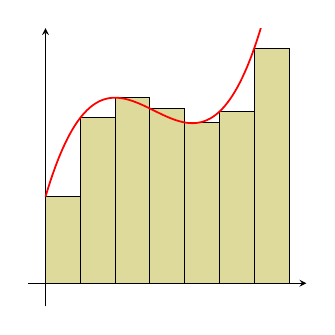
\begin{tikzpicture}[scale=0.8]
        \begin{axis}[
            axis lines=middle,
            xtick=\empty,
            ytick=\empty,
            xmin=-0.5, xmax=7.5,
            ymin=-0.5, ymax=5.5,
            width=6cm, height=6cm
        ]
        \addplot[ybar interval, fill=olive!30, domain=0:7, samples=8] {0.1 * (x-2)^3- 1/3 * (x-2)^2 + 4};
        \addplot[domain=0:7, samples=100, color=red, thick] {0.1 * (x-2)^3- 1/3 * (x-2)^2 + 4};
        \end{axis}
    \end{tikzpicture}
    \hspace{1cm}
    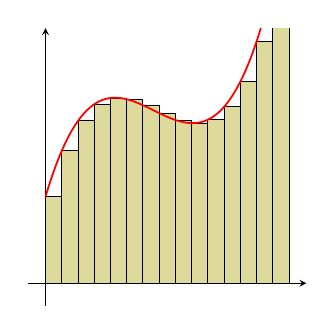
\begin{tikzpicture}[scale=0.8]
        \begin{axis}[
            axis lines=middle,
            xtick=\empty,
            ytick=\empty,
            xmin=-0.5, xmax=7.5,
            ymin=-0.5, ymax=5.5,
            width=6cm, height=6cm
        ]
        \addplot[ybar interval, fill=olive!30, domain=0:7, samples=16] {0.1 * (x-2)^3- 1/3 * (x-2)^2 + 4};
        \addplot[domain=0:7, samples=100, color=red, thick] {0.1 * (x-2)^3- 1/3 * (x-2)^2 + 4};
        \end{axis}
    \end{tikzpicture}
    \caption{Xấp xỉ diện tích bằng các hình chữ nhật.}
    \label{fig:rectangle_approx}
\end{figure}
\begin{figure}[H]
    \centering
    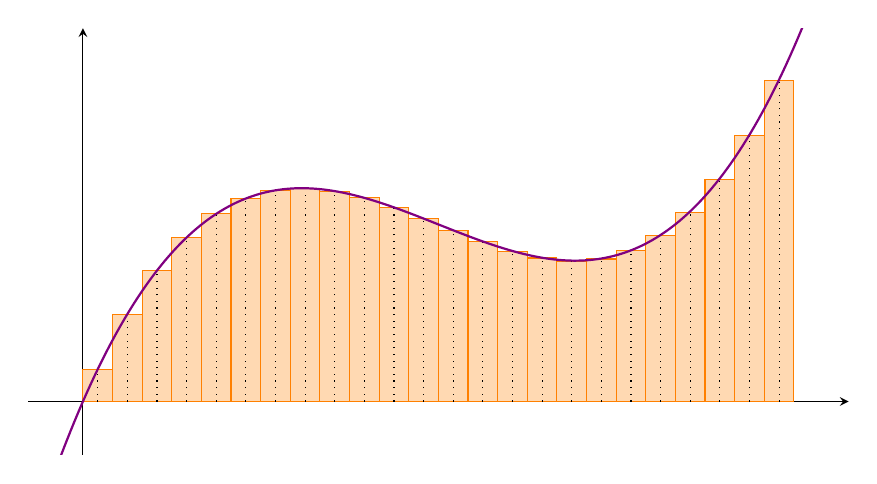
\begin{tikzpicture}[scale=1]
        \begin{axis}[
            axis lines=middle,
            xtick=\empty,
            ytick=\empty,
            xmin=-1, xmax=14,
            ymin=-1, ymax=7,
            width=12cm, height=7cm
        ]
        
        % Số cột
        \pgfmathsetmacro{\N}{24}
        % Bước chia
        \pgfmathsetmacro{\dx}{13/\N}
        
        % Vẽ các cột Riemann (lấy theo trung điểm)
        \foreach \i in {0,...,23} {
            \pgfmathsetmacro{\xmid}{(\i+0.5)*\dx} % trung điểm
            \pgfmathsetmacro{\y}{1/46*\xmid^3 - 39/92*\xmid^2 + 54/23*\xmid}
            % Hình chữ nhật (cột)
            \addplot[ybar, bar width=\dx, fill=orange!30, draw=orange] coordinates {(\xmid, \y)};
            % Đường chấm dọc
            \addplot[dotted, black] coordinates {(\xmid,0) (\xmid,\y)};
        }

        % Vẽ đường cong màu tím
        \addplot[domain=-0.8:13.5, samples=200, color=violet, thick] {1/46*x^3 - 39/92*x^2 + 54/23*x};
        
        \end{axis}
    \end{tikzpicture}
    \caption{Tổng Riemann (lấy theo trung điểm).}
    \label{fig:riemann_sum}
\end{figure}


\begin{example}
    Xét hàm số $f$ xác định bởi $f(x) = x^4 + 2$ trên đoạn $[1, 5]$. Ta sẽ tính xấp xỉ diện tích của miền dưới đồ thị hàm $f$.
    
    Ta xây dựng biểu thức tổng Riemann của $f$ trên $[1, 5]$ bằng cách chia đoạn này thành 8 đoạn con có độ dài bằng nhau, và chọn điểm mẫu là trung điểm của mỗi đoạn.
    
    Độ dài của mỗi đoạn con là $\Delta x = \dfrac{5-1}{8} = \dfrac{1}{2}$. Các điểm chia là $x_i = 1 + \dfrac{5-1}{8}i = 1 + \dfrac{i}{2}$ với $1 \le i \le 8$. Trung điểm của mỗi đoạn con $[x_{i-1}, x_i]$ là $x_i^* = 1 + \dfrac{5-1}{8}(i-1) + \dfrac{5-1}{16} = \dfrac{7}{8} + \dfrac{i}{2}$. Tổng Riemann tương ứng là:
    \[ \sum_{i=1}^{8} f(x_i^*) \Delta x = \sum_{i=1}^{8} \dfrac{1}{2} \left[ \left(\dfrac{7}{8} + \dfrac{i}{2}\right)^4 + 2 \right] \approx 645.34 \]
    Đây là một giá trị xấp xỉ cho diện tích của miền dưới đồ thị hàm $f(x) = x^4 + 2$ trên đoạn $[1, 5]$.
\end{example}

\begin{example}
    Một ô tô di chuyển trên một đường thẳng, với vận tốc tức thời tại thời điểm $t$ (đơn vị là km/h) là $v(t)$. Dữ liệu về vận tốc được ghi lại sau mỗi 15 phút như trong bảng sau:
    \begin{center}
    \begin{tabular}{|c|c|c|c|c|c|c|}
        \hline
        $t$ (giờ) & 0 & 0.25 & 0.5 & 0.75 & 1 & 1.25 \\
        \hline
        $v(t)$ (km/h) & 40 & 65 & 80 & 70 & 90 & 85 \\
        \hline
    \end{tabular}
    \end{center}
    Hãy ước lượng quãng đường mà ô tô đã đi được.

    Trên mỗi khoảng thời gian $[t_{i-1}, t_i]$, ta có thể xấp xỉ quãng đường đi được bằng cách lấy vận tốc ở đầu khoảng thời gian nhân với độ dài của khoảng thời gian đó: $v(t_{i-1})(t_i - t_{i-1})$. Tổng quãng đường đi được ước tính là:
    \[ 40 \cdot 0.25 + 65 \cdot 0.25 + 80 \cdot 0.25 + 70 \cdot 0.25 + 90 \cdot 0.25 = 86.25 \text{ km}. \]
    
    Tương tự, ta có thể xấp xỉ bằng cách sử dụng vận tốc ở cuối mỗi khoảng thời gian:
    \[ 65 \cdot 0.25 + 80 \cdot 0.25 + 70 \cdot 0.25 + 90 \cdot 0.25 + 85 \cdot 0.25 = 97.5 \text{ km}. \]
    Hai cách tính cho ra hai kết quả khác nhau. Ta hy vọng rằng có một giá trị chính xác cho quãng đường, và các giá trị trên chỉ là những xấp xỉ. Khi ta thu thập dữ liệu với các khoảng thời gian nhỏ hơn, các giá trị xấp xỉ sẽ tiến gần hơn đến giá trị thực.
\end{example}

\begin{example}
    Tốc độ quang hợp của một loài thực vật, ký hiệu là $P$, được đo bằng lượng $CO_2$ (tính bằng micromol trên mét vuông mỗi giây) mà lá cây hấp thụ. Dữ liệu thu thập được tại các thời điểm $t$ (tính bằng giây) như sau:
    \begin{center}
    \begin{tabular}{|c|c|c|c|c|c|c|}
        \hline
        $t$ & 0 & 15 & 30 & 45 & 60 & 75 \\
        \hline
        $P(t)$ & 3.1 & 4.5 & 5.2 & 6.1 & 5.8 & 5.3 \\
        \hline
    \end{tabular}
    \end{center}
    Ta muốn tính tổng lượng $CO_2$ mà một mét vuông lá cây hấp thụ được trong 75 giây đầu tiên.
    
    Nếu ta sử dụng giá trị đo ở đầu mỗi khoảng thời gian làm đại diện, ta có ước lượng:
    \[ 3.1 \cdot 15 + 4.5 \cdot 15 + 5.2 \cdot 15 + 6.1 \cdot 15 + 5.8 \cdot 15 = 370.5 \text{ micromol/m}^2. \]
    
    Nếu ta sử dụng giá trị đo ở cuối mỗi khoảng, ta có:
    \[ 4.5 \cdot 15 + 5.2 \cdot 15 + 6.1 \cdot 15 + 5.8 \cdot 15 + 5.3 \cdot 15 = 396 \text{ micromol/m}^2. \]
    Các ví dụ trên minh họa cho một ý tưởng chung: để tính một \textbf{tổng giá trị} của hàm $f$ trên một đoạn $I = [a, b]$, ta có thể chia nhỏ $I$ thành các đoạn con. Trên mỗi đoạn con, sự thay đổi của hàm $f$ sẽ ít hơn, do đó ta có thể xấp xỉ $f$ bằng một hằng số, chẳng hạn giá trị $f(x_i^*)$ tại một điểm mẫu. Tổng giá trị của $f$ trên đoạn $[x_{i-1}, x_i]$ được xấp xỉ bởi $f(x_i^*)(x_i - x_{i-1})$, và do đó, tổng giá trị trên toàn bộ đoạn $I$ được xấp xỉ bởi tổng Riemann:
    \[ \sum_{i=1}^{n} f(x_i^*) (x_i - x_{i-1}). \]
    Ta kỳ vọng rằng khi phép chia đoạn càng mịn (các đoạn con càng nhỏ), giá trị xấp xỉ sẽ càng tốt hơn, và giới hạn của quá trình này sẽ cho ta giá trị chính xác.
\end{example}

Để hiểu ``giới hạn'' của tổng Riemann một cách chính xác, ta nói rằng giới hạn đó là một số thực $L$ mà mọi tổng Riemann đều có thể tiến gần đến $L$ một cách tùy ý, miễn là phép chia đủ mịn.

\begin{definition}
    Giả sử tồn tại một số thực $L$ sao cho với mọi số thực $\epsilon > 0$, có một số thực $\delta > 0$ để với mọi phép chia
    \[ a = x_0 < x_1 < x_2 < \dots < x_n = b \]
    mà độ dài của mỗi đoạn $[x_{i-1}, x_i]$ đều nhỏ hơn $\delta$, và với mọi cách chọn điểm mẫu $x_i^* \in [x_{i-1}, x_i]$, ta luôn có:
    \[ \left| \sum_{i=1}^{n} f(x_i^*) (x_i - x_{i-1}) - L \right| < \epsilon. \]
    Số thực $L$ (nếu tồn tại) là duy nhất và được gọi là \textbf{tích phân} của $f$ trên $[a, b]$, ký hiệu là
    \[ \int_{a}^{b} f \quad \text{hoặc} \quad \int_{a}^{b} f(x) \dd x. \]
\end{definition}

Ký hiệu $\dd x$ trong tích phân chủ yếu để chỉ rõ biến số lấy tích phân và thường không có ý nghĩa độc lập. Nếu tích phân của $f$ tồn tại, ta nói hàm $f$ \textbf{có tích phân} hoặc \textbf{khả tích}. Khi $f$ khả tích, ta có thể tính xấp xỉ tích phân của nó với độ chính xác mong muốn bằng cách tính tổng Riemann.

\begin{definition}
    Nếu hàm $f$ không âm và khả tích trên đoạn $[a, b]$, ta định nghĩa \textbf{diện tích} của miền phẳng nằm dưới đồ thị của $f$ và trên trục $x$ là:
    \[ \int_{a}^{b} f(x) \dd x. \]
\end{definition}

% TODO: Sửa lại tham chiếu
Chúng ta sẽ quay lại vấn đề diện tích một cách chi tiết hơn trong Mục  \ref{sec:integral_applications}. Ta mở rộng định nghĩa của ký hiệu tích phân như sau. Với $a < b$, ta định nghĩa:
\[ \int_{b}^{a} f(x) \dd x = - \int_{a}^{b} f(x) \dd x. \]
Và ta cũng quy ước:
\[ \int_{a}^{a} f(x) \dd x = 0. \]

\subsection{Tính chất của tích phân}

Các tính chất sau đây được suy ra trực tiếp từ định nghĩa của tích phân thông qua tổng Riemann.

\begin{proposition} (Các tính chất cơ bản của tích phân)
    \begin{enumerate}[label=(\alph*)]
        \item Tích phân nếu tồn tại thì là duy nhất.
        
        \item Nếu $k$ là một hằng số thực và hàm $f$ có tích phân thì hàm $kf$ cũng có tích phân và
        \[ \int_{a}^{b} [k f(x)] \dd x = k \int_{a}^{b} f(x) \dd x. \]
        
        \item Nếu các hàm $f$ và $g$ đều có tích phân thì tổng $f+g$ cũng có tích phân và
        \[ \int_{a}^{b} [f(x) + g(x)] \dd x = \int_{a}^{b} f(x) \dd x + \int_{a}^{b} g(x) \dd x. \]
        
        \item Nếu hàm $f$ có tích phân trên các đoạn $[a, c]$ và $[c, b]$ thì $f$ cũng có tích phân trên $[a, b]$ và
        \[ \int_{a}^{c} f(x) \dd x + \int_{c}^{b} f(x) \dd x = \int_{a}^{b} f(x) \dd x. \]
        
        \item Nếu $f(x) \ge g(x)$ với mọi $x \in [a, b]$ thì
        \[ \int_{a}^{b} f(x) \dd x \ge \int_{a}^{b} g(x) \dd x. \]
    \end{enumerate}
\end{proposition}

Một số tính chất này có thể được giải thích và minh họa một cách trực quan thông qua ý nghĩa hình học. Chẳng hạn, tính chất (d) có thể hiểu là diện tích miền dưới đồ thị của $f$ trên đoạn $[a, b]$ bằng tổng diện tích trên các đoạn $[a, c]$ và $[c, b]$. Tương tự, tính chất (e) cho thấy nếu đồ thị của $f$ cao hơn đồ thị của $g$, thì diện tích tương ứng cũng lớn hơn.

\begin{proof}
    (a) Các tổng Riemann không thể cùng lúc tiến gần đến hai số thực khác nhau.
    
    (b) Đặt $\int_a^b f(x) \dd x = M$. Khi tổng Riemann của $f$ tiến gần đến $M$ một cách tùy ý, thì tổng Riemann của $kf$ cũng sẽ tiến gần đến $kM$ một cách tùy ý.
    
    (c) Đặt $\int_a^b g(x) \dd x = N$. Ta xét tổng Riemann của $f+g$ như sau, với $\Delta x_i = x_i - x_{i-1}$:
    \begin{align*}
        \left| \sum_{i} (f(x_i^*) + g(x_i^*))\Delta x_i - (M+N) \right| &= \left| \left(\sum_i f(x_i^*)\Delta x_i - M\right) + \left(\sum_i g(x_i^*)\Delta x_i - N\right) \right| \\
        &\le \left| \sum_i f(x_i^*)\Delta x_i - M \right| + \left| \sum_i g(x_i^*)\Delta x_i - N \right|.
    \end{align*}
    Điều này cho thấy nếu tổng Riemann của $f$ gần $M$ và tổng Riemann của $g$ gần $N$ thì tổng Riemann của $f+g$ sẽ gần $M+N$.
    
    (e) Nếu $f \ge g$ thì mọi tổng Riemann của $f$ sẽ lớn hơn hoặc bằng tổng Riemann tương ứng của $g$, tức là $\sum_i f(x_i^*)\Delta x_i \ge \sum_i g(x_i^*)\Delta x_i$.
\end{proof}

Từ cách xây dựng tích phân, có thể thấy rằng tính liên tục của hàm là một điều kiện rất quan trọng để đảm bảo phép xấp xỉ có hiệu quả. Nói một cách đơn giản, tính liên tục đảm bảo rằng khi biến số thay đổi nhỏ thì giá trị của hàm cũng thay đổi nhỏ, nhờ đó việc xấp xỉ giá trị hàm bằng cách lấy một giá trị đại diện trở nên chính xác hơn. Kết quả dưới đây khẳng định rằng tất cả các hàm liên tục đều khả tích.

\begin{theorem}[Hàm liên tục thì có tích phân]
    Nếu hàm $f$ liên tục trên đoạn $[a, b]$ thì tích phân $\int_a^b f$ tồn tại.
\end{theorem}

Có thể tìm thấy chứng minh chi tiết mệnh đề trên trong các tài liệu như
[TPTT02], [Spi94].

\subsection{Bài tập}

\begin{exercise}
    Một người đi xe đạp ghi lại vận tốc của mình (mét/giây) tại các thời điểm khác nhau (giây) trong 10 giây đầu tiên như sau:
    \begin{center}
    \begin{tabular}{|c|c|c|c|c|c|c|}
        \hline
        $t$ (giây) & 0 & 2 & 4 & 6 & 8 & 10 \\
        \hline
        $v(t)$ (m/s) & 0 & 1.5 & 2.5 & 3.0 & 2.5 & 2.0 \\
        \hline
    \end{tabular}
    \end{center}
    Hãy ước tính tổng quãng đường người đó đi được bằng hai cách:
    \begin{enumerate}[label=(\alph*)]
        \item Sử dụng vận tốc ở đầu mỗi khoảng thời gian (tổng Riemann trái).
        \item Sử dụng vận tốc ở cuối mỗi khoảng thời gian (tổng Riemann phải).
    \end{enumerate}
\end{exercise}

\begin{exercise}
    Cho hàm số $f$ liên tục trên đoạn $[0, 8]$. Bảng dưới đây cung cấp một số giá trị của hàm $f$:
    \begin{center}
    \begin{tabular}{|c|c|c|c|c|c|}
        \hline
        $x$ & 0 & 2 & 4 & 6 & 8 \\
        \hline
        $f(x)$ & 1.2 & 2.8 & 4.0 & 3.5 & 2.0 \\
        \hline
    \end{tabular}
    \end{center}
    Hãy tính xấp xỉ tích phân $\int_{0}^{8} f(x) \dd x$ bằng cách sử dụng tổng Riemann với 4 đoạn con có độ dài bằng nhau và lấy điểm mẫu là điểm cuối bên phải của mỗi đoạn.
\end{exercise}

\begin{exercise}
    Hãy tính tổng Riemann cho hàm số $f(x) = x^4$ trên đoạn $[0, 1]$ bằng cách chia đoạn này thành 5 đoạn con có độ dài bằng nhau và chọn điểm mẫu là trung điểm của mỗi đoạn.
\end{exercise}

\begin{exercise}
    Tính tổng Riemann cho hàm số $f(x) = \cos(\frac{\pi x}{8})$ trên đoạn $[0, 4]$, sử dụng 8 đoạn con có độ dài bằng nhau và lấy điểm mẫu là điểm đầu bên trái của mỗi đoạn.
\end{exercise}

\begin{exercise}
    Dựa vào đồ thị của hàm số $f$ trong hình dưới đây, hãy ước lượng diện tích của miền giới hạn bởi đồ thị và trục hoành trên đoạn $[0, 5]$.
    \begin{figure}[H]
        \centering
        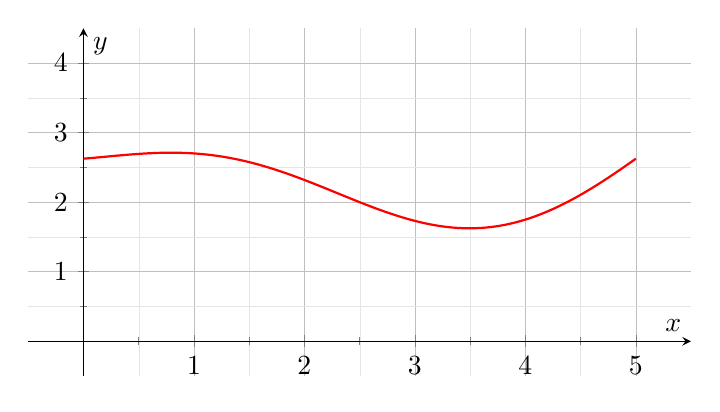
\begin{tikzpicture}[scale=1]
            \begin{axis}[
                axis lines=middle,
                grid=both,
                minor tick num=1,
                grid style={line width=.1pt, draw=gray!20},
                major grid style={line width=.2pt,draw=gray!50},
                xtick={0,1,2,3,4,5},
                ytick={0,1,2,3,4},
                xmin=-0.5, xmax=5.5,
                ymin=-0.5, ymax=4.5,
                width=10cm, height=6cm,
                xlabel=$x$,
                ylabel=$y$
            ]
            \addplot[domain=0:5, samples=100, color=red, thick, smooth] {2 + 0.5*sin(deg(x*pi/2.5)) + 0.1*(x-2.5)^2};
            \end{axis}
        \end{tikzpicture}
        \caption{Đồ thị của hàm số $f$ cho Bài tập 5.1.5.}
    \end{figure}
\end{exercise}

\begin{exercise}
    Sử dụng các tính chất của tích phân để chứng minh bất đẳng thức sau mà không cần tính giá trị của các tích phân:
    \[ \int_{0}^{1} \sqrt{1+x^2} \dd x \le \int_{0}^{1} \sqrt{1+x} \dd x. \]
    Gợi ý: So sánh hai hàm số $x^2$ và $x$ trên đoạn $[0, 1]$.
\end{exercise}

\begin{exercise}
    Sử dụng tính chất so sánh của tích phân để kiểm tra ước lượng sau:
    \[ 2 \le \int_{-1}^{1} \sqrt{1+x^4} \dd x \le 2\sqrt{2}. \]
\end{exercise}

\begin{exercise}
    Tìm một chặn trên và một chặn dưới cho tích phân sau:
    \[ \int_{0}^{2} \frac{1}{x^3+1} \dd x. \]
\end{exercise}

\begin{exercise}[*]
    Giả sử $f$ là một hàm liên tục trên đoạn $[a, b]$ và $f(x) \ge 0$ với mọi $x \in [a, b]$. Hãy giải thích tại sao nếu $\int_{a}^{b} f(x) \dd x = 0$ thì ta phải có $f(x) = 0$ với mọi $x \in [a, b]$.
\end{exercise}

\begin{exercise}
    Theo định luật Hooke, lực cần thiết để kéo dãn một lò xo thêm $x$ đơn vị so với chiều dài tự nhiên của nó là $F(x) = kx$, trong đó $k$ là hằng số lò xo. Giả sử một lò xo có chiều dài tự nhiên là 20 cm. Nếu cần một lực 50 N để giữ lò xo ở chiều dài 30 cm, hãy tính công thực hiện khi kéo lò xo từ chiều dài 30 cm đến 40 cm.
    
    (Gợi ý: Công được tính bằng tích phân của lực theo quãng đường dịch chuyển, $W = \int_a^b F(x) \dd x$).
\end{exercise}

\section{Định lý Cơ bản của phép tính vi tích phân}

\subsection{Nguyên hàm}
Phép lấy nguyên hàm là phép toán ngược của phép lấy đạo hàm. Nếu $F$ là đạo hàm của $f$, ta nói $F$ là một \textbf{nguyên hàm} của $f$.

\begin{example}
    Vì $(x)' = 1$, hàm $F(x) = x$ là một nguyên hàm của hàm $f(x)=1$. Tương tự, vì $(x+5)'=1$, hàm $G(x) = x+5$ cũng là một nguyên hàm khác của $f$.
\end{example}

\begin{proposition}
    Nếu $F$ là một nguyên hàm của $f$ trên khoảng $(a,b)$, thì tất cả các nguyên hàm khác của $f$ trên khoảng đó đều có dạng $F(x) + C$, trong đó $C$ là một hằng số thực.
\end{proposition}
\begin{proof}
    Giả sử $G$ là một nguyên hàm bất kỳ khác của $f$. Khi đó, ta có $(F-G)' = F' - G' = f - f = 0$.
    Do đó, theo Hệ quả 4.1.13, hàm $F-G$ phải là một hàm hằng, tức là $F(x) - G(x) = C$ với mọi $x \in (a,b)$.
\end{proof}

Nếu hàm $f$ có nguyên hàm, tập hợp tất cả các nguyên hàm của $f$ được gọi là \textbf{tích phân bất định} của $f$, và được ký hiệu là
\[ \int f(x) \dd x. \]
Theo quy ước, ta thường viết tập hợp này dưới dạng:
\[ \int f(x) \dd x = F(x) + C, \]
trong đó $F$ là một nguyên hàm cụ thể của $f$ và $C$ đại diện cho một hằng số tùy ý.

\begin{example}
    Một số nguyên hàm cơ bản:
    \begin{enumerate}[label=(\alph*)]
        \item $\int k \dd x = kx + C$ (với $k$ là hằng số).
        \item $\int x^n \dd x = \dfrac{x^{n+1}}{n+1} + C$ (với $n \neq -1$).
        \item Từ $(\ln|x|)' = \dfrac{1}{x}$, ta có $\int \dfrac{1}{x} \dd x = \ln|x| + C$.
        \item $\int e^x \dd x = e^x + C$. Tổng quát hơn, $\int e^{kx} \dd x = \dfrac{1}{k}e^{kx} + C$ (với $k \neq 0$).
        \item $\int \dfrac{1}{\sqrt{1-x^2}} \dd x = \arcsin x + C$.
        \item $\int \dfrac{1}{1+x^2} \dd x = \arctan x + C$.
    \end{enumerate}
\end{example}

\begin{proposition}[Tính tuyến tính của nguyên hàm]
    Nếu $f$ và $g$ có nguyên hàm, thì $f+g$ và $k \cdot f$ (với $k$ là hằng số) cũng có nguyên hàm, và:
    \[ \int [f(x) + g(x)] \dd x = \int f(x) \dd x + \int g(x) \dd x \]
    \[ \int [k \cdot f(x)] \dd x = k \int f(x) \dd x \]
\end{proposition}

\begin{example}
    Áp dụng tính tuyến tính để tính nguyên hàm của một đa thức:
    \begin{align*}
        \int (6x^2 - 8x + 3) \dd x &= 6 \int x^2 \dd x - 8 \int x \dd x + \int 3 \dd x \\
        &= 6 \left(\frac{x^3}{3}\right) - 8 \left(\frac{x^2}{2}\right) + 3x + C \\
        &= 2x^3 - 4x^2 + 3x + C.
    \end{align*}
\end{example}

\subsection{Công thức Newton-Leibniz và Định lý Cơ bản}

Định lý sau đây thiết lập một cầu nối vô cùng quan trọng giữa hai nhánh chính của giải tích: phép tính vi phân và phép tính tích phân.

\begin{theorem}[Định lý Cơ bản của Phép tính Vi tích phân, Phần 1] \label{thm:FTC1}
    Nếu hàm $f$ liên tục trên đoạn $[a, b]$ thì hàm $F$ được định nghĩa bởi
    \[ F(x) = \int_{a}^{x} f(t) \dd t, \quad a \le x \le b \]
    là một nguyên hàm của $f$ trên $[a,b]$. Do đó,
    \begin{importantbox}
        \[ \dfrac{\dd}{\dd x} \int_{a}^{x} f(t) \dd t = f(x). \]
    \end{importantbox}
\end{theorem}

Định lý này khẳng định rằng mọi hàm liên tục đều có nguyên hàm. Nó cho thấy rằng phép lấy đạo hàm của một tích phân sẽ trả về hàm số ban đầu, chứng tỏ phép tính vi phân và tích phân là hai quá trình ngược nhau.

Về mặt hình học, Định lý \ref{thm:FTC1} có thể được giải thích một cách trực quan. Nếu $f \ge 0$, thì $F(x)$ biểu diễn diện tích miền dưới đồ thị của $f$ từ $a$ đến $x$. Phần diện tích tăng thêm khi $x$ tăng một lượng nhỏ $h$, tức $F(x+h) - F(x)$, có thể được xấp xỉ bằng diện tích của một hình chữ nhật có chiều cao $f(x)$ và chiều rộng $h$.
\[ F(x+h) - F(x) \approx f(x) \cdot h \implies \dfrac{F(x+h) - F(x)}{h} \approx f(x). \]
Khi $h \to 0$, phép xấp xỉ này trở nên chính xác và ta có $F'(x) = f(x)$.

\begin{figure}[H]
    \centering
    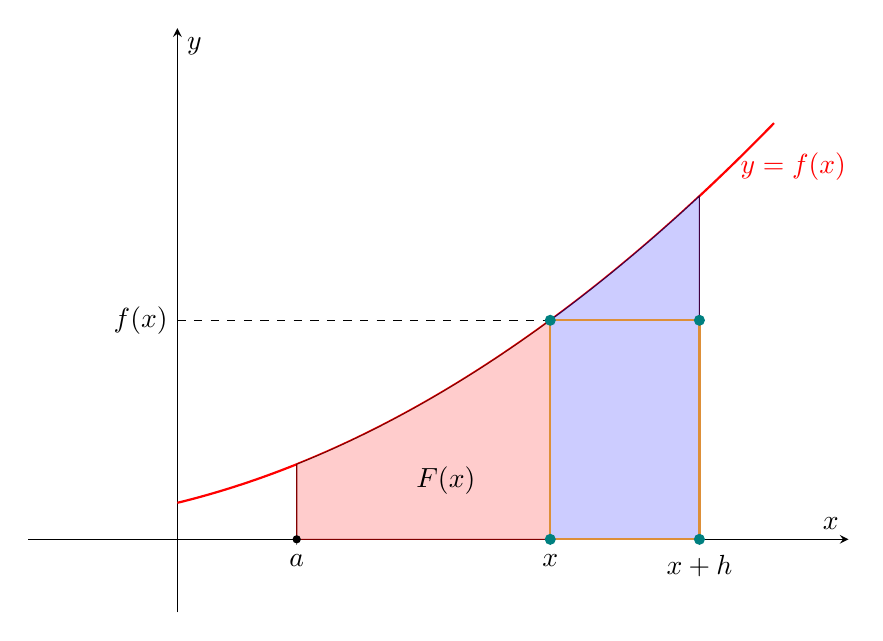
\begin{tikzpicture}
        \begin{axis}[
            axis lines=middle,
            xlabel=$x$,
            ylabel=$y$,
            xtick={0.8, 2.5, 3.5},
            xticklabels={$a$, $x$, $x+h$},
            ytick=\empty,
            xmin=-1, xmax=4.5,
            ymin=-1, ymax=7,
            width=12cm,
            height=9cm,
            clip=false,
            % Khai báo hàm f(x) để vẽ
            declare function={
                myfunc(\t) = 0.2*\t^2 + 0.5*\t + 0.5;
            }
        ]
        
        % Tọa độ các điểm chính
        \coordinate (a) at (axis cs:0.8,0);
        \coordinate (x) at (axis cs:2.5,0);
        \coordinate (x_h) at (axis cs:3.5,0);
        \coordinate (f_x) at (axis cs:2.5, {myfunc(2.5)});
        \coordinate (f_x_h) at (axis cs:3.5, {myfunc(3.5)});
        
        % 1. Vẽ đồ thị hàm số y=f(x)
        \addplot[
            domain=0:4, 
            samples=100, 
            color=red, 
            thick
        ] {myfunc(x)} node[pos=0.9, right] {$y=f(x)$};
        
        % 2. Tô màu vùng F(x) (màu đỏ nhạt)
        \addplot[
            fill=red!20,
            draw=black!50!red,
            domain=0.8:2.5,
        ] {myfunc(x)} \closedcycle;
        \node at (axis cs:1.8, 0.8) {$F(x)$};
        
        % 3. Tô màu vùng F(x+h) - F(x) (màu xanh lá nhạt)
        \addplot[
            fill=blue!20,
            draw=black!50!violet,
            domain=2.5:3.5,
        ] {myfunc(x)} \closedcycle;

        % 4. Vẽ hình chữ nhật màu vàng bên trong vùng màu xanh
        \draw[thick, draw=yellow!50!purple] (axis cs:2.5,0) rectangle (axis cs:3.5, {myfunc(2.5)});

        % 5. Vẽ các đường gióng và nhãn
        % Đường gióng từ x tới f(x)
        \draw[dashed] (axis cs:0, {myfunc(2.5)}) node[left] {$f(x)$} -- (f_x);
        
        % Các điểm chấm trên đồ thị
        \fill[teal] (f_x) circle (2pt);
        % \fill[blue] (f_x_h) circle (2pt);
        \fill[teal] (axis cs:3.5, {myfunc(2.5)}) circle (2pt);
        
        % Các điểm chấm trên trục hoành
        \fill[teal] (x) circle (2pt);
        \fill[teal] (x_h) circle (2pt);
        \fill (a) circle (1.5pt);

        \end{axis}
    \end{tikzpicture}
    \caption{\centering Xấp xỉ tuyến tính của sự gia tăng diện tích. Diện tích của dải hẹp $\Delta F = F(x+h) - F(x)$ có giá trị gần bằng diện tích hình chữ nhật đáy $h$ và chiều cao $f(x)$.}
    \label{fig:fundamental-theorem-1}
\end{figure}

\begin{proof}
    Chứng minh dưới đây là cách hình thức hóa lý luận hình học ở trên. Theo định nghĩa đạo hàm, ta có:
    \[ F'(x) = \limit{h}{0} \dfrac{F(x+h) - F(x)}{h} = \limit{h}{0} \dfrac{1}{h} \int_{x}^{x+h} f(t) \dd t. \]
    Ta biến đổi biểu thức bên trong giới hạn:
    \[ \dfrac{1}{h} \int_{x}^{x+h} f(t) \dd t - f(x) = \dfrac{1}{h} \int_{x}^{x+h} [f(t) - f(x)] \dd t. \]
    Vì $f$ liên tục tại $x$, với mọi $\epsilon > 0$, tồn tại $\delta > 0$ sao cho nếu $|h| < \delta$ thì $|f(t) - f(x)| < \epsilon$ với mọi $t$ nằm giữa $x$ và $x+h$. Do đó:
    \[ \left| \dfrac{1}{h} \int_{x}^{x+h} [f(t) - f(x)] \dd t \right| \le \dfrac{1}{|h|} \int_{x}^{x+h} |f(t) - f(x)| \dd t < \dfrac{1}{|h|} |h| \epsilon = \epsilon. \]
    Điều này chứng tỏ $\limit{h}{0} \dfrac{1}{h} \int_{x}^{x+h} f(t) \dd t = f(x)$. Vậy $F'(x) = f(x)$.
\end{proof}

\begin{example}
    Áp dụng trực tiếp Định lý Cơ bản của Phép tính Vi tích phân:
    \[ \dfrac{\dd}{\dd x} \int_{0}^{x} t^2 \dd t = x^2. \]
\end{example}

\begin{example}
    Để tìm đạo hàm của $h(x) = \int_{1}^{\sqrt{x}} \dfrac{z^2}{z^4+1} \dd z$, ta sử dụng quy tắc chuỗi.
    Đặt $u = \sqrt{x}$ và $F(u) = \int_{1}^{u} \dfrac{z^2}{z^4+1} \dd z$.
    Khi đó $h(x) = F(u(x))$. Theo quy tắc chuỗi và Định lý \ref{thm:FTC1}:
    \[ h'(x) = F'(u) \cdot u'(x) = \dfrac{u^2}{u^4+1} \cdot \dfrac{1}{2\sqrt{x}} = \dfrac{(\sqrt{x})^2}{(\sqrt{x})^4+1} \cdot \dfrac{1}{2\sqrt{x}} = \dfrac{x}{x^2+1} \cdot \dfrac{1}{2\sqrt{x}}. \]
\end{example}

\begin{example}
    Xét một vật chuyển động thẳng với vận tốc tức thời tại thời điểm $t$ là $v(t)$. Quãng đường vật đi được từ thời điểm $a$ đến $t$ là $s(t) = \int_a^t v(u) \dd u$.
    Định lý Cơ bản của Phép tính Vi tích phân cho ta:
    \[ s'(t) = \dfrac{\dd}{\dd t} \int_a^t v(u) \dd u = v(t). \]
    Kết quả này hoàn toàn phù hợp với định nghĩa vật lý rằng vận tốc là đạo hàm của quãng đường (hay vị trí) theo thời gian.
\end{example}

\begin{example}
    Hàm \textbf{sai số} (error function), ký hiệu $\mathrm{erf}(x)$, là một hàm quan trọng trong xác suất và thống kê, được định nghĩa bằng một tích phân:
    \[ \mathrm{erf}(x) = \dfrac{2}{\sqrt{\pi}} \int_{0}^{x} e^{-t^2} \dd t. \]
    Theo Định lý Cơ bản, đạo hàm của nó là $\mathrm{erf}'(x) = \dfrac{2}{\sqrt{\pi}} e^{-x^2}$. Đồ thị của hàm $e^{-x^2}$ có dạng hình chuông (đường cong Gauss) kinh điển.
    
    \begin{figure}[H]
        \centering
        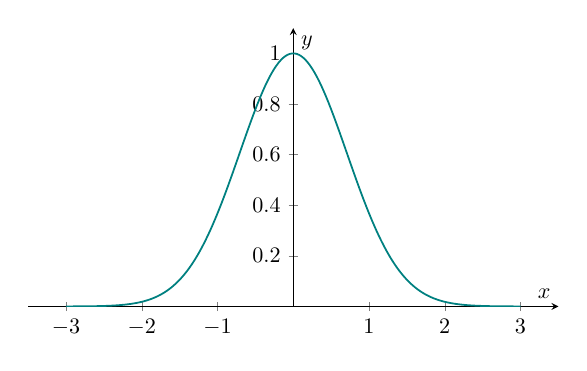
\begin{tikzpicture}[scale=0.8]
            \begin{axis}[
                axis lines=middle,
                samples=200,
                domain=-3:3,
                ytick={0.2, 0.4, 0.6, 0.8, 1.0},
                xmin=-3.5, xmax=3.5,
                ymin=0, ymax=1.1,
                xlabel=$x$,
                ylabel=$y$,
                width=10cm, height=6cm
            ]
            \addplot[color=teal, thick] {exp(-x^2)};
            \end{axis}
        \end{tikzpicture}
        \caption{Đồ thị hình chuông của hàm $e^{-x^2}$.}
    \end{figure}
\end{example}


\begin{theorem} (Công thức Newton-Leibniz)
    Nếu $f$ là hàm liên tục trên đoạn $[a, b]$ và $F$ là một nguyên hàm bất kỳ của $f$ trên đoạn đó, thì
    \begin{importantbox}
    \[ \int_{a}^{b} f(x) \dd x = F(b) - F(a) = \left.F(x)\right|_a^b. \]
    \end{importantbox}
\end{theorem}

Công thức Newton-Leibniz cung cấp một phương pháp vô cùng hiệu quả để tính tích phân xác định: thay vì phải tính giới hạn phức tạp của tổng Riemann, ta chỉ cần tìm một nguyên hàm của hàm số và tính hiệu các giá trị của nó tại hai đầu mút của đoạn tích phân.

Có thể giải thích gần đúng Công thức Newton-Leibniz bằng tổng Riemann như sau. Với bất kì phép chia nào của đoạn $[a, b]$ bởi $a = x_0 < x_1 < \dots < x_n = b$, vì
\[ F(x_i) - F(x_{i-1}) \approx F'(x_{i-1})(x_i - x_{i-1}) = f(x_{i-1})\Delta x_i \]
nên tổng Riemann tương ứng của hàm $f$ là
\[ \sum_{i=1}^{n} f(x_{i-1})\Delta x_i \approx \sum_{i=1}^{n} (F(x_i) - F(x_{i-1})) = F(x_n) - F(x_0) = F(b) - F(a). \]
Dẫn tới $\int_a^b f(x) \dd x \approx F(b) - F(a)$.

Một cách trực quan hơn, giả sử $a < b$ và $f \ge 0$. Ta dùng ý nghĩa tích phân $\int_a^b f(x) \dd x$ là diện tích bên dưới đồ thị của $f$ trên đoạn $[a, b]$, và lấy $F(x)$ là diện tích bên dưới đồ thị trên đoạn $[a, x]$. Khi đó, $F(a) = 0$ và $F(b)$ bằng diện tích trên toàn đoạn $[a, b]$, nên hiển nhiên $\int_a^b f(x) \dd x = F(b) - F(a)$. Từ Định lý Cơ bản của Phép tính Vi tích phân (Phần 1), ta đã biết $F$ là một nguyên hàm của $f$, và vì hai nguyên hàm bất kì của $f$ chỉ khác nhau một hằng số, nên để tính hiệu số $F(b) - F(a)$ ta dùng nguyên hàm nào cũng được. Đây cũng là nội dung của chứng minh bên dưới.

\begin{proof}
    Theo Định lý Cơ bản của Phép tính Vi tích phân (Phần 1) \ref{thm:FTC1}, hàm
    \[ G(x) = \int_a^x f(t) \dd t \]
    là một nguyên hàm của $f$. Ta có ngay $G(a) = \int_a^a f(t) \dd t = 0$, và
    \[ G(b) - G(a) = G(b) = \int_a^b f(t) \dd t. \]
    Bây giờ, giả sử $F$ là một nguyên hàm bất kỳ khác của $f$. Khi đó, tồn tại hằng số $C$ sao cho $F(x) = G(x) + C$ (theo Mệnh đề 5.2.2). Ta có:
    \[ F(b) - F(a) = (G(b)+C) - (G(a)+C) = G(b) - G(a) = \int_a^b f(t) \dd t. \]
    Điều này cho thấy kết quả không phụ thuộc vào việc chọn nguyên hàm cụ thể.
\end{proof}

\begin{example}
    Ta tính dễ dàng bằng Công thức Newton–Leibniz:
    \[ \int_{0}^{1} x \dd x = \left. \frac{1}{2}x^2 \right|_0^1 = \frac{1}{2}(1)^2 - \frac{1}{2}(0)^2 = \frac{1}{2}. \]
\end{example}

\begin{example}
    Tiếp tục Ví dụ 5.2.13, ta xét một vật chuyển động theo một chiều thẳng, với tốc độ tức thời tại thời điểm $t$ là $v(t)$ biến đổi liên tục. Chiều dài quãng đường đi được của vật từ thời điểm $a$ tới thời điểm $t$ cho bởi tích phân
    \[ s(t) = \int_a^t v(u) \dd u. \]
    Lấy một điểm nào đó trên đường làm điểm gốc, thì vị trí của xe ở thời điểm $t$ cho bởi số thực $x(t)$. Vì vận tốc là đạo hàm của vị trí theo thời gian, $v(t) = x'(t)$, nên Công thức Newton–Leibniz cho chiều dài quãng đường đi được của vật từ thời điểm $a$ tới thời điểm $t$ bằng
    \[ s(t) = \int_a^t v(u) \dd u = x(t) - x(a). \]
    Đây cũng chính là lượng thay đổi vị trí của chiếc xe (ta đang giả thiết vật chỉ di chuyển theo một chiều, không đổi chiều), và như vậy không phụ thuộc vào cách chọn điểm gốc. Ta cũng có $s(t) = x(t) - x(a)$ với mọi $t$, tức là chiều dài quãng đường đi được và vị trí chỉ sai khác một hằng số. Đặc biệt nếu tốc độ chuyển động là hằng $v$ (chuyển động thẳng đều) thì ta thu lại công thức quen thuộc $x(b) - x(a) = v(b - a)$, tức là chiều dài đường đi bằng tốc độ đi nhân thời gian đi.
\end{example}

% TODO: Sửa lại tham chiếu
\begin{figure}[H]
    \centering
    \begin{tikzpicture}
        % Dòng thời gian
        \draw[->, thick, blue!60] (-1,0) -- (11,0) node[right] {thời gian};
        \fill[blue!60] (3,0) circle (2pt) node[above] {$a$};
        \fill[blue!60] (6,0) circle (2pt) node[above] {$t$};
        \fill[blue!60] (7.8,0) circle (2pt) node[above] {$b$};

        % Dòng vị trí
        \draw[->, thick, orange!80!black] (-1,1) -- (11,1) node[right] {$x$};
        \fill[orange!80!black] (0,1) circle (2pt) node[above] {0};
        \fill[orange!80!black] (2,1) circle (2pt) node[above] {$x(a)$};
        \fill[orange!80!black] (6,1) circle (2pt) node[above] {$x(t)$};
        \fill[orange!80!black] (8.5,1) circle (2pt) node[above] {$x(b)$};

        % Chú thích quãng đường s(t)
        \draw[<->, thick, green!60!black] (2, 2) -- (6, 2) node[midway, above] {$s(t)$};
    \end{tikzpicture}
    \caption{Vị trí và quãng đường trong chuyển động thẳng một chiều.}
    \label{fig:position_distance_v2}
\end{figure}

Trong sách giáo khoa trung học [SGKTHPT], tích phân xác định thường được định nghĩa bằng Công thức Newton-Leibniz, tiện cho tính toán nhưng khó thấy được ý nghĩa và ứng dụng.

\subsection{Bài tập}

\begin{exercise}
    Tính các tích phân xác định sau:
    \begin{enumerate}[label=(\alph*)]
        \item $\int_{1}^{3} (\sqrt{x} - \frac{2}{\sqrt[3]{x^2}} + x) \dd x$.
        \item $\int_{-2}^{2} |x^2 - 1| \dd x$.
        \item $\int_{0}^{\pi} |\cos x| \dd x$.
        \item $\int_{-1}^{2} f(x) \dd x$ với $f(x) = \begin{cases} x^3, & \text{nếu } -1 \le x < 1, \\ x^4, & \text{nếu } 1 \le x \le 2. \end{cases}$
    \end{enumerate}
\end{exercise}

\begin{exercise}
    Sử dụng Định lý Cơ bản của Phép tính Vi tích phân để tìm đạo hàm của các hàm số sau:
    \begin{enumerate}[label=(\alph*)]
        \item $g(x) = \int_{2}^{x} \sqrt{1+t^4} \dd t$.
        \item $h(x) = \int_{x}^{10} \ln(z^2+1) \dd z$.
        \item $F(x) = \int_{1}^{x^3} \cos(t) \dd t$.
        \item $G(x) = \int_{\sin x}^{\cos x} (1+v^2)^{10} \dd v$.
    \end{enumerate}
\end{exercise}

\begin{exercise}
    Cho hàm số $f(x) = \int_{0}^{x^2} \ln(t^2 + e) \dd t$. Hãy tính $f'(1)$.
\end{exercise}

\begin{exercise}
    Bằng cách lấy đạo hàm vế phải, hãy chứng minh các công thức nguyên hàm sau:
    \begin{enumerate}[label=(\alph*)]
        \item \[\int \dfrac{1}{x^2 \sqrt{1 + x^2}} = - \dfrac{\sqrt{1 + x^2}}{x} + C\]. 
        \item \[\int \frac{1}{x \sqrt{1-x^2}} \dd x = -\ln\left(\frac{1+\sqrt{1-x^2}}{x}\right) + C\].
        \item \[\int \frac{x^2}{\sqrt{a^2-x^2}} \dd x = \frac{a^2}{2}\arcsin\left(\frac{x}{a}\right) - \frac{x}{2}\sqrt{a^2-x^2} + C\].
    \end{enumerate}
\end{exercise}

\begin{exercise}
    Tính giá trị của biểu thức tích phân lồng nhau sau:
    \[ \int_{0}^{1} \left( \int_{1}^{y} e^{x^2} \dd x \right) \dd y. \]
    (Gợi ý: Đặt $F(y) = \int_{1}^{y} e^{x^2} \dd x$ và sử dụng tích phân từng phần).
\end{exercise}

\begin{exercise}
    Khảo sát sự thay đổi của tích phân $I_n = \int_0^1 x^n \dd x$ khi số nguyên dương $n$ tăng. Hãy giải thích kết quả bằng cách phác họa đồ thị của hàm $y=x^n$ với một vài giá trị của $n$.
\end{exercise}

\begin{exercise}
    Một bể chứa ban đầu có 500 lít nước. Nước được bơm vào bể với tốc độ $v(t) = 200 - 8t$ (lít/phút), trong đó $t$ là thời gian tính bằng phút kể từ lúc bắt đầu bơm. Hỏi sau 10 phút, lượng nước trong bể là bao nhiêu?
\end{exercise}

\begin{exercise}
    Lưu lượng giao thông tại một nút giao thông được mô hình hóa bởi hàm $f(t) = -400t^2 + 2400t + 4000$ (xe/giờ), với $t=0$ tương ứng với 7 giờ sáng. Hãy tính tổng số xe đi qua nút giao này trong khoảng thời gian từ 8 giờ sáng ($t=1$) đến 10 giờ sáng ($t=3$).
\end{exercise}

\begin{exercise}
    Dòng chảy của một con sông mang theo bùn. Tốc độ lắng đọng của bùn tại một vị trí nhất định được cho bởi hàm $d(t) = 10 \sqrt{t} + \frac{t^2}{100}$ (kg/ngày), với $t$ là thời gian tính bằng ngày. Hãy tính tổng khối lượng bùn lắng đọng trong 100 ngày đầu tiên.
\end{exercise}

\begin{exercise}
    Công suất tiêu thụ điện của một nhà máy (tính bằng megawatt, MW) được mô hình hóa bởi hàm $P(t) = 2t^2 + 30$, với $t$ là số giờ kể từ 6 giờ sáng. Hãy tính tổng năng lượng điện (tính bằng megawatt-giờ) mà nhà máy tiêu thụ trong khoảng thời gian từ 8 giờ sáng ($t=2$) đến 4 giờ chiều ($t=10$).
\end{exercise}

\begin{exercise}
    Cho hàm số $f(x) = \int_{0}^{x} \frac{(t-4)^2 e^t}{\sqrt{t^2+9}} \dd t$, với $x \in [0, 5]$. Hãy xác định giá trị của $x$ để $f(x)$ đạt giá trị nhỏ nhất.
\end{exercise}

\section{Các phương pháp biến đổi và tính tích phân}

\subsection{Phép đổi biến trong tích phân}
\begin{theorem}
    Giả sử $u = g(x)$ là một hàm khả vi liên tục trên một khoảng $I$ và hàm $f$ liên tục trên tập giá trị của $g$. Khi đó trên $I$, ta có:
    \[ \int f(g(x))g'(x) \dd x = \int f(u) \dd u. \]
\end{theorem}
\begin{proof}
    Vì $f$ liên tục trên $I$ nên nó có một nguyên hàm $F$, do đó $\int f(u) \dd u = F(u) + C$. Theo quy tắc đạo hàm hàm hợp, ta có:
    \[
        (F \circ g)'(x) = F'(g(x))g'(x) = f(g(x))g'(x).
    \]
    Điều này cho thấy $F \circ g$ là một nguyên hàm của hàm $x \mapsto f(g(x))g'(x)$. Do đó:
    \[
        \int f(g(x))g'(x) \dd x = F(g(x)) + D = F(u) + D = \int f(u) \dd u.
    \]
\end{proof}

Sau đây là phiên bản của phương pháp thế cho tích phân xác định.
\begin{theorem}[Công thức đổi biến]
    Giả sử $u = g(x)$ là hàm khả vi liên tục trên $[a, b]$, và $f$ liên tục trên tập giá trị của $g$. Khi đó:
    \begin{equation}
        \int_a^b f(g(x))g'(x) \dd x = \int_{g(a)}^{g(b)} f(u) \dd u.
    \end{equation}
\end{theorem}
\begin{proof}
    Gọi $F$ là một nguyên hàm bất kỳ của $f$. Khi đó, $F(g(x))$ là một nguyên hàm của $f(g(x))g'(x)$. Áp dụng Công thức Newton-Leibniz, ta có:
    \[
        \int_a^b f(g(x))g'(x) \dd x = F(g(x))\bigg|_a^b = F(g(b)) - F(g(a)) = \int_{g(a)}^{g(b)} f(u) \dd u.
    \]
\end{proof}

\begin{example}
    Tính $\int x \sin(x^2 + 3) \dd x$.
\end{example}
\begin{solution}
    Ta thực hiện phép thế $u = x^2+3$, suy ra $\dd u = 2x \dd x$, hay $x \dd x = \frac{1}{2}\dd u$. Tích phân trở thành:
    \[
        \int x \sin(x^2 + 3) \dd x = \int \sin(u) \left(\frac{1}{2}\dd u\right) = \frac{1}{2}\int \sin u \dd u = -\frac{1}{2}\cos u + C.
    \]
    Thay $u$ trở lại theo $x$, ta được kết quả:
    \[
        \int x \sin(x^2 + 3) \dd x = -\frac{1}{2}\cos(x^2+3) + C.
    \]
\end{solution}

\begin{example}
    Tính $\int_0^1 \dfrac{x}{1+x^2} \dd x$.
\end{example}
\begin{solution}
    Đặt $u = 1+x^2$, suy ra $\dd u = 2x \dd x$, hay $x\dd x = \frac{1}{2}\dd u$. Ta đổi cận tích phân: khi $x=0$ thì $u=1+0^2=1$, và khi $x=1$ thì $u=1+1^2=2$. Tích phân trở thành:
    \[
        \int_0^1 \dfrac{x}{1+x^2} \dd x = \int_1^2 \dfrac{1}{u} \left(\dfrac{1}{2}\dd u\right) = \dfrac{1}{2} \int_1^2 \dfrac{1}{u}\dd u = \dfrac{1}{2}\ln\abs{u}\bigg|_1^2 = \dfrac{1}{2}(\ln 2 - \ln 1) = \dfrac{1}{2}\ln 2.
    \]
\end{solution}

Tóm lại, quy trình đổi biến có thể được thực hiện theo các bước sau:
\begin{importantbox}
    \textbf{Phương pháp đổi biến trong tích phân}
    \begin{itemize}
        \item \textbf{Bước 1:} Chọn một biểu thức phù hợp để đặt biến mới, thường là $u = g(x)$.
        \item \textbf{Bước 2:} Tính vi phân $\dd u = g'(x) \dd x$.
        \item \textbf{Bước 3:} Đối với tích phân xác định, đổi cận tích phân từ biến $x$ sang biến $u$.
        \item \textbf{Bước 4:} Viết lại tích phân theo biến $u$ và giải. Nếu là tích phân bất định, hãy thay biến $u$ trở lại theo $x$ ở kết quả cuối cùng.
    \end{itemize}

\end{importantbox}

\begin{proposition}[Tính đối xứng của tích phân]
    Giả sử hàm $f$ liên tục trên đoạn $[-a, a]$.
    \begin{enumerate}[label=(\alph*)]
        \item Nếu $f$ là hàm chẵn, tức là $f(-x) = f(x)$, thì $\int_{-a}^a f(x) \dd x = 2 \int_0^a f(x) \dd x$.
        \item Nếu $f$ là hàm lẻ, tức là $f(-x) = -f(x)$, thì $\int_{-a}^a f(x) \dd x = 0$.
    \end{enumerate}
\end{proposition}
\begin{proof}
    Ta tách tích phân ban đầu thành hai phần:
    \[
        \int_{-a}^a f(x) \dd x = \int_{-a}^0 f(x) \dd x + \int_0^a f(x) \dd x.
    \]
    Trong tích phân thứ nhất, ta đổi biến $u = -x$. Khi đó $\dd u = -\dd x$. Cận tích phân đổi từ $x=-a \Rightarrow u=a$ và $x=0 \Rightarrow u=0$.
    \[
        \int_{-a}^0 f(x) \dd x = \int_{a}^{0} f(-u) (-\dd u) = \int_0^a f(-u) \dd u.
    \]
    Kết hợp lại, ta có:
    \[
        \int_{-a}^a f(x) \dd x = \int_0^a f(-u) \dd u + \int_0^a f(x) \dd x.
    \]
    Nếu $f$ là hàm chẵn, $f(-u) = f(u)$, và tích phân trở thành $2 \int_0^a f(x) \dd x$. Nếu $f$ là hàm lẻ, $f(-u) = -f(u)$, và tích phân trở thành $0$.
\end{proof}

\subsection{Tích phân từng phần}
Từ quy tắc đạo hàm của tích hai hàm số $f$ và $g$:
\[
    \deriv{}{x}[f(x)g(x)] = f(x)g'(x) + g(x)f'(x).
\]
Lấy nguyên hàm hai vế, ta có:
\[
    f(x)g(x) = \int f(x)g'(x) \dd x + \int g(x)f'(x) \dd x.
\]
Sắp xếp lại, ta được công thức \textbf{tích phân từng phần} cho tích phân bất định:
\begin{importantbox}
    \[ \int f(x)g'(x) \dd x = f(x)g(x) - \int g(x)f'(x) \dd x. \]
\end{importantbox}
Đặt $u = f(x)$ và $v = g(x)$, ta có $\dd u = f'(x)\dd x$ và $\dd v = g'(x)\dd x$. Công thức trên có dạng rút gọn và dễ nhớ:
\begin{importantbox}
    \[ \int u \dd v = uv - \int v \dd u. \]
\end{importantbox}
Đối với tích phân xác định, công thức tương ứng là:
\begin{importantbox}
    \[ \int_a^b f(x)g'(x) \dd x = f(x)g(x)\bigg|_a^b - \int_a^b g(x)f'(x) \dd x. \]
\end{importantbox}

\begin{example}
    Tính $\int x \cos x \dd x$.
\end{example}
\begin{solution}
    Ta sử dụng phương pháp tích phân từng phần. Đặt:
    \[
        u = x \implies \dd u = \dd x
    \]
    \[
        \dd v = \cos x \dd x \implies v = \sin x
    \]
    Áp dụng công thức, ta có:
    \begin{align*}
        \int x \cos x \dd x &= x \sin x - \int \sin x \dd x \\
        &= x \sin x - (-\cos x) + C \\
        &= x \sin x + \cos x + C.
    \end{align*}
\end{solution}

\begin{example}
    Tính $\int x^2 \ln x \dd x$.
\end{example}
\begin{solution}
    Đặt:
    \[
        u = \ln x \implies \dd u = \dfrac{1}{x} \dd x
    \]
    \[
        \dd v = x^2 \dd x \implies v = \dfrac{x^3}{3}
    \]
    Áp dụng công thức tích phân từng phần:
    \begin{align*}
        \int x^2 \ln x \dd x &= \dfrac{x^3}{3} \ln x - \int \dfrac{x^3}{3} \cdot \dfrac{1}{x} \dd x \\
        &= \dfrac{x^3}{3} \ln x - \int \dfrac{x^2}{3} \dd x \\
        &= \dfrac{x^3}{3} \ln x - \dfrac{x^3}{9} + C.
    \end{align*}
\end{solution}

\begin{example}
    Tính $\int_0^{\pi/2} e^x \sin x \dd x$.
\end{example}
\begin{solution}
    Ta áp dụng tích phân từng phần hai lần. Đặt $I = \int_0^{\pi/2} e^x \sin x \dd x$. \\
    Lần 1: Đặt $u = \sin x, \dd v = e^x \dd x$. Ta có $\dd u = \cos x \dd x, v = e^x$.
    \[
        I = e^x \sin x \bigg|_0^{\pi/2} - \int_0^{\pi/2} e^x \cos x \dd x = e^{\pi/2} - \int_0^{\pi/2} e^x \cos x \dd x.
    \]
    Lần 2: Tính $J = \int_0^{\pi/2} e^x \cos x \dd x$. Đặt $u' = \cos x, \dd v' = e^x \dd x$. Ta có $\dd u' = -\sin x \dd x, v' = e^x$.
    \[
        J = e^x \cos x \bigg|_0^{\pi/2} - \int_0^{\pi/2} e^x (-\sin x) \dd x = (0 - 1) + \int_0^{\pi/2} e^x \sin x \dd x = -1 + I.
    \]
    Thay $J$ vào biểu thức của $I$, ta có:
    \[
        I = e^{\pi/2} - (-1 + I) = e^{\pi/2} + 1 - I.
    \]
    Suy ra $2I = e^{\pi/2} + 1$, vậy $I = \dfrac{e^{\pi/2} + 1}{2}$.
\end{solution}

\subsection{Một số phương pháp tính tích phân đặc biệt}

\subsubsection{Tích phân của hàm lượng giác}

\begin{example}
    Tính $\int \cos^3 x \dd x$.
\end{example}
\begin{solution}
    Ta có thể tính tích phân này bằng cách tách $\cos x$ và sử dụng phép đổi biến $u = \sin x$.
    \begin{align*}
        \int \cos^3 x \dd x &= \int \cos^2 x \cos x \dd x \\
        &= \int (1 - \sin^2 x) \cos x \dd x \\
        &= \int (1 - u^2) \dd u \quad (\text{với } u = \sin x, \dd u = \cos x \dd x) \\
        &= u - \dfrac{1}{3}u^3 + C \\
        &= \sin x - \dfrac{1}{3}\sin^3 x + C.
    \end{align*}
\end{solution}

%% Ghi chú: Ví dụ gốc (5.3.11) đã được thay đổi từ ∫sin⁵x cos²x dx thành ∫sin³x cos⁴x dx để tránh sao chép.
%% Phương pháp giải cốt lõi (tách sin x và đổi biến u = cos x) được bảo toàn.
\begin{example}
    Tính $\int \sin^3 x \cos^4 x \dd x$.
\end{example}
\begin{solution}
    Ta đổi biến $u = \cos x$, suy ra $\dd u = -\sin x \dd x$.
    \begin{align*}
        \int \sin^3 x \cos^4 x \dd x &= \int \sin^2 x \cos^4 x \sin x \dd x \\
        &= \int (1 - \cos^2 x) \cos^4 x \sin x \dd x \\
        &= \int (1 - u^2)u^4 (-\dd u) \\
        &= -\int (u^4 - u^6) \dd u \\
        &= -\left( \dfrac{u^5}{5} - \dfrac{u^7}{7} \right) + C \\
        &= \dfrac{1}{7}\cos^7 x - \dfrac{1}{5}\cos^5 x + C.
    \end{align*}
\end{solution}

%% Ghi chú: Ví dụ gốc (5.3.12) đã được thay đổi từ ∫sin⁴x dx thành ∫cos⁴x dx để tránh sao chép.
%% Phương pháp giải cốt lõi (sử dụng công thức hạ bậc) được bảo toàn.
\begin{example}
    Tính $\int \cos^4 x \dd x$.
\end{example}
\begin{solution}
    Ta sử dụng công thức hạ bậc $\cos^2 x = \dfrac{1 + \cos(2x)}{2}$.
    \begin{align*}
        \int \cos^4 x \dd x &= \int \left(\cos^2 x\right)^2 \dd x \\
        &= \int \left( \dfrac{1 + \cos(2x)}{2} \right)^2 \dd x \\
        &= \dfrac{1}{4} \int \left( 1 + 2\cos(2x) + \cos^2(2x) \right) \dd x \\
        &= \dfrac{1}{4} \int \left( 1 + 2\cos(2x) + \dfrac{1 + \cos(4x)}{2} \right) \dd x \\
        &= \dfrac{1}{4} \int \left( \dfrac{3}{2} + 2\cos(2x) + \dfrac{1}{2}\cos(4x) \right) \dd x \\
        &= \dfrac{1}{4} \left( \dfrac{3}{2}x + \sin(2x) + \dfrac{1}{8}\sin(4x) \right) + C.
    \end{align*}
\end{solution}

Các hệ thức lượng giác sau đây có thể hữu ích cho việc tính tích phân các tích của hàm sin và cos:
\begin{align*}
    \sin A \cos B &= \dfrac{1}{2}[\sin(A - B) + \sin(A + B)] \\
    \sin A \sin B &= \dfrac{1}{2}[\cos(A - B) - \cos(A + B)] \\
    \cos A \cos B &= \dfrac{1}{2}[\cos(A - B) + \cos(A + B)]
\end{align*}

\subsubsection{Các phép đổi biến lượng giác}
Một số phép đổi biến lượng giác thường dùng, với hàm $\sec\theta = \dfrac{1}{\cos\theta}$:
\begin{center}
    \begin{tabular}{|c|c|c|}
        \hline
        \textbf{Biểu thức} & \textbf{Phép đổi biến} & \textbf{Hệ thức} \\
        \hline
        $\sqrt{a^2 - x^2}$ & $x = a \sin\theta$ & $1 - \sin^2\theta = \cos^2\theta$ \\
        \hline
        $\sqrt{a^2 + x^2}$ & $x = a \tan\theta$ & $1 + \tan^2\theta = \sec^2\theta$ \\
        \hline
        $\sqrt{x^2 - a^2}$ & $x = a \sec\theta$ & $\sec^2\theta - 1 = \tan^2\theta$ \\
        \hline
        $x^2 + a^2$ & $x = a \tan\theta$ & $dx = a \sec^2\theta d\theta$ \\
        \hline
        $x^2 - a^2$ & $x = a \sec\theta$ & $dx = a \sec\theta \tan\theta d\theta$ \\
        \hline
    \end{tabular}
\end{center}

%% Ghi chú: Ví dụ gốc (5.3.13) đã được thay đổi từ ∫√(9 - x²) dx thành ∫√(16 - x²) dx để tránh sao chép.
%% Phương pháp giải cốt lõi (đổi biến x = a sinθ) được bảo toàn.
\begin{example}
    Tính $\int \sqrt{16 - x^2} \dd x$.
\end{example}
\begin{solution}
    Đặt $x = 4\sin\theta$, với $-\dfrac{\pi}{2} \le \theta \le \dfrac{\pi}{2}$. Khi đó $\dd x = 4\cos\theta \dd\theta$.
    Do điều kiện của $\theta$, ta có $\cos\theta \ge 0$, nhờ đó $\sqrt{16 - 16\sin^2\theta} = \sqrt{16\cos^2\theta} = 4\cos\theta$.
    \begin{align*}
        \int \sqrt{16 - x^2} \dd x &= \int (4\cos\theta)(4\cos\theta) \dd\theta \\
        &= 16 \int \cos^2\theta \dd\theta \\
        &= 16 \int \dfrac{1 + \cos(2\theta)}{2} \dd\theta \\
        &= 8 \left(\theta + \dfrac{1}{2}\sin(2\theta) \right) + C \\
        &= 8\theta + 4\sin(2\theta) + C \\
        &= 8\theta + 8\sin\theta\cos\theta + C.
    \end{align*}
    Từ $x = 4\sin\theta$, ta có $\theta = \arcsin\left(\dfrac{x}{4}\right)$ và $\cos\theta = \sqrt{1 - \sin^2\theta} = \sqrt{1 - \left(\dfrac{x}{4}\right)^2} = \dfrac{\sqrt{16 - x^2}}{4}$.
    Thay vào kết quả trên, ta được:
    \[
        \int \sqrt{16 - x^2} \dd x = 8\arcsin\left(\dfrac{x}{4}\right) + 8\left(\dfrac{x}{4}\right)\dfrac{\sqrt{16 - x^2}}{4} + C = 8\arcsin\left(\dfrac{x}{4}\right) + \dfrac{x\sqrt{16-x^2}}{2} + C.
    \]
\end{solution}

\subsubsection{Tích phân của hàm hữu tỉ}
Ta minh họa phương pháp qua một số ví dụ sau.

%% Ghi chú: Ví dụ gốc (5.3.14) đã được thay đổi từ ∫(x³+x)/(x-1) dx thành ∫(x³+2x)/(x-1) dx để tránh sao chép.
\begin{example}
    Tính $\int \dfrac{x^3+2x}{x-1} \dd x$.
\end{example}
\begin{solution}
    Ta thực hiện phép chia đa thức:
    \begin{align*}
        \int \dfrac{x^3+2x}{x-1} \dd x &= \int \left(x^2 + x + 3 + \dfrac{3}{x-1}\right) \dd x \\
        &= \dfrac{x^3}{3} + \dfrac{x^2}{2} + 3x + 3\ln\abs{x-1} + C.
    \end{align*}
\end{solution}

%% Ghi chú: Ví dụ gốc (5.3.15) đã được thay đổi để tránh sao chép. Kỹ thuật phân tích thành phân thức đơn giản được giữ lại.
\begin{example}
    Tính $\int \dfrac{x+4}{x^2 - 5x + 6} \dd x$.
\end{example}
\begin{solution}
    Ta có thể phân tích hàm dưới dấu tích phân thành tổng sau:
    \[
        \dfrac{x+4}{x^2 - 5x + 6} = \dfrac{x+4}{(x-2)(x-3)} = \dfrac{A}{x-2} + \dfrac{B}{x-3}.
    \]
    Giải đồng nhất thức ta được $A = -6$ và $B = 7$. Vì vậy:
    \begin{align*}
        \int \dfrac{x+4}{x^2 - 5x + 6} \dd x &= \int \left( \dfrac{-6}{x-2} + \dfrac{7}{x-3} \right) \dd x \\
        &= -6\ln\abs{x-2} + 7\ln\abs{x-3} + C.
    \end{align*}
\end{solution}

%% Ghi chú: Ví dụ gốc (5.3.16) đã được thay đổi để tránh sao chép. Kỹ thuật phân tích với mẫu chứa nhân tử bậc hai bất khả quy được giữ lại.
\begin{example}
    Tính $\int \dfrac{3x^2-x+6}{x^3+3x} \dd x$.
\end{example}
\begin{solution}
    \begin{align*}
        \int \dfrac{3x^2-x+6}{x(x^2+3)} \dd x &= \int \left( \dfrac{2}{x} + \dfrac{x-1}{x^2+3} \right) \dd x \\
        &= \int \dfrac{2}{x} \dd x + \int \dfrac{x}{x^2+3} \dd x - \int \dfrac{1}{x^2+3} \dd x \\
        &= 2\ln\abs{x} + \dfrac{1}{2}\ln(x^2+3) - \dfrac{1}{\sqrt{3}}\arctan\left(\dfrac{x}{\sqrt{3}}\right) + K.
    \end{align*}
\end{solution}

%% Ghi chú: Ví dụ gốc (5.3.17) đã được thay đổi để tránh sao chép. Kỹ thuật chia đa thức và hoàn thành bình phương ở mẫu được giữ lại.
\begin{example}
    Tính $\int \dfrac{2x^2-x+4}{x^2-2x+5} \dd x$.
\end{example}
\begin{solution}
    Ta chia đa thức và được:
    \[
        \dfrac{2x^2-x+4}{x^2-2x+5} = 2 + \dfrac{3x-6}{x^2-2x+5}.
    \]
    Chú ý rằng $x^2-2x+5 = (x-1)^2+4$. Ta đổi biến $u=x-1$, suy ra $\dd u = \dd x$ và $x=u+1$.
    \begin{align*}
        \int \dfrac{2x^2-x+4}{x^2-2x+5} \dd x &= \int \left( 2 + \dfrac{3x-6}{(x-1)^2+4} \right) \dd x \\
        &= 2x + \int \dfrac{3(u+1)-6}{u^2+4} \dd u \\
        &= 2x + \int \dfrac{3u-3}{u^2+4} \dd u \\
        &= 2x + 3\int \dfrac{u}{u^2+4} \dd u - 3\int \dfrac{1}{u^2+4} \dd u \\
        &= 2x + \dfrac{3}{2}\ln(u^2+4) - \dfrac{3}{2}\arctan\left(\dfrac{u}{2}\right) + C \\
        &= 2x + \dfrac{3}{2}\ln(x^2-2x+5) - \dfrac{3}{2}\arctan\left(\dfrac{x-1}{2}\right) + C.
    \end{align*}
\end{solution}

\subsection{Sự tồn tại công thức cho tích phân}

Theo Định lý cơ bản của Vi tích phân, mọi hàm liên tục đều có nguyên hàm được cho bởi một tích phân. Do đó, câu hỏi về việc ``tính'' tích phân của một hàm thực chất là tìm một công thức tường minh cho nguyên hàm đó. ``Công thức tường minh'' ở đây có nghĩa chính xác là một biểu thức được tạo nên từ các hàm số sơ cấp.

Tuy nhiên, sau này người ta đã chứng minh được rằng có những hàm liên tục mà nguyên hàm của chúng không phải là hàm sơ cấp. Do đó, không thể biểu diễn tích phân của chúng bằng một công thức tường minh.

\begin{example}
    Hàm số $f(x) = e^{x^2}$ là một hàm liên tục trên $\R$ và do đó có nguyên hàm. Tuy nhiên, người ta đã chứng minh được rằng nguyên hàm của nó không thể biểu diễn dưới dạng một hàm sơ cấp. Một số tích phân khác cũng được biết là không có nguyên hàm sơ cấp bao gồm:
    \[ \int \dfrac{e^x}{x}\dd x, \quad \int \sin(x^2)\dd x, \quad \int \cos(e^x)\dd x, \quad \int \sqrt{x^3+1}\dd x, \quad \int \dfrac{1}{\ln x}\dd x, \quad \int \dfrac{\sin x}{x}\dd x. \]
\end{example}

Việc tìm công thức tường minh cho nguyên hàm nói chung vẫn là một bài toán khó, mặc dù đã được nghiên cứu từ rất lâu. Trong nhiều trường hợp, công thức không tồn tại hoặc quá phức tạp để sử dụng. Do đó, người ta thường dùng các phương pháp khác để khảo sát tích phân, chẳng hạn như phân tích thành chuỗi, tính toán xấp xỉ, hoặc biến đổi để khảo sát các tính chất mà không cần đến công thức tường minh.

\subsubsection{Tính tích phân bằng phần mềm máy tính}

Việc tính toán tích phân thường phức tạp và mỗi loại hàm đòi hỏi những phương pháp riêng. Các hệ Đại số Máy tính (Computer Algebra Systems - CAS) hiện đại thường được cài đặt các thuật toán rất mạnh để tìm nguyên hàm, trong đó có thuật toán Risch, cho phép xác định một hàm cho trước có nguyên hàm sơ cấp hay không và nếu có thì sẽ đưa ra công thức của nó.

\begin{example}
    Tính $\int \sqrt{\cot x} \dd x$.
\end{example}
\begin{solution}
    Sử dụng phần mềm máy tính như WolframAlpha hoặc Maxima, ta có thể thu được một kết quả rất phức tạp, cho thấy việc tính toán bằng tay sẽ rất khó khăn:
    \[
        -\dfrac{1}{\sqrt{2}}\ln(\cos x - \sqrt{2\sin x \cos x} + \sin x) + \dfrac{1}{\sqrt{2}}\ln(\cos x + \sqrt{2\sin x \cos x} + \sin x) + C.
    \]
\end{solution}

\subsection{Tính tích phân bằng phương pháp số}

Trong nhiều trường hợp, việc tính chính xác giá trị tích phân là không thể hoặc không cần thiết. Hơn nữa, có những hàm số được cho dưới dạng bảng dữ liệu từ thực nghiệm và không có công thức tường minh. Khi đó, việc tính xấp xỉ tích phân là mối quan tâm chính.

Phương pháp cơ bản là sử dụng một tổng Riemann với cách chia khoảng và chọn điểm đại diện thích hợp. Dưới đây ta xét phương pháp xấp xỉ dựa trên cách chia đều miền xác định. Cho hàm $f$ xác định trên $[a, b]$, ta chia đoạn này thành $n$ khoảng con bằng nhau, mỗi khoảng có chiều dài $\Delta x = \dfrac{b-a}{n}$. Đặt $x_i = a + i\Delta x$, $0 \le i \le n$.

\begin{importantbox}
    \textbf{Quy tắc điểm giữa (Midpoint Rule)} \\
    Lấy tổng Riemann với điểm đại diện là trung điểm của mỗi khoảng con, ta có công thức xấp xỉ:
    \[
        \int_a^b f(x) \dd x \approx M_n = [f(x_1^*) + f(x_2^*) + \dots + f(x_n^*)]\Delta x
    \]
    với $x_i^* = \dfrac{1}{2}(x_{i-1} + x_i)$.
\end{importantbox}

\begin{example}
    Sử dụng Quy tắc điểm giữa với $n = 4$ để xấp xỉ $\int_1^2 \dfrac{1}{x} \dd x$.
\end{example}
\begin{solution}
    Đoạn $[1, 2]$ được chia thành 4 khoảng con, mỗi khoảng có chiều rộng $\Delta x = \dfrac{2-1}{4} = 0.25$.
    Các điểm chia là $1, 1.25, 1.5, 1.75, 2$.
    Các trung điểm tương ứng là $1.125, 1.375, 1.625, 1.875$.
    Theo Quy tắc điểm giữa:
    \begin{align*}
        \int_1^2 \dfrac{1}{x} \dd x &\approx M_4 = 0.25 \left[ f(1.125) + f(1.375) + f(1.625) + f(1.875) \right] \\
        &= 0.25 \left( \dfrac{1}{1.125} + \dfrac{1}{1.375} + \dfrac{1}{1.625} + \dfrac{1}{1.875} \right) \\
        &\approx 0.25 (0.8888... + 0.7272... + 0.6153... + 0.5333...) \\
        &\approx 0.6912.
    \end{align*}
    Giá trị chính xác của tích phân là $\ln(2) \approx 0.6931$.
\end{solution}

Ngoài ra, còn có những phương pháp xấp xỉ khác như \textbf{Quy tắc hình thang} (xấp xỉ bằng hình thang) hay \textbf{Quy tắc Simpson} (xấp xỉ bằng đường parabol). Các đề tài này thường được khảo sát sâu hơn trong môn Phương pháp tính hay Giải tích số.

\subsection{Tích phân suy rộng}

Có những câu hỏi đơn giản như diện tích bên dưới đồ thị của hàm $y = \dfrac{1}{x}$ trên khoảng $(1, \infty)$ bằng bao nhiêu? Để trả lời những câu hỏi như vậy ta xây dựng khái niệm \textbf{tích phân suy rộng}, ở đó cận tích phân có thể là $\pm\infty$ hoặc hàm số không bị chặn tại cận.

\begin{definition}(Tích phân suy rộng) Với $a,b \in \R$
    \begin{enumerate}[label=(\alph*)]
        \item Nếu $\int_a^t f(x) \dd x$ tồn tại với mọi $t \ge a$, ta định nghĩa:
        \[ \int_a^\infty f(x) \dd x = \lim_{t \to \infty} \int_a^t f(x) \dd x. \]
        \item Nếu $\int_t^b f(x) \dd x$ tồn tại với mọi $t \le b$, ta định nghĩa:
        \[ \int_{-\infty}^b f(x) \dd x = \lim_{t \to -\infty} \int_t^b f(x) \dd x. \]
        \item Nếu $\int_{-\infty}^c f(x) \dd x$ và $\int_c^\infty f(x) \dd x$ cùng hội tụ với một số $c$ nào đó, ta định nghĩa:
        \[ \int_{-\infty}^\infty f(x) \dd x = \int_{-\infty}^c f(x) \dd x + \int_c^\infty f(x) \dd x. \]
        \item Nếu $f$ liên tục trên $(a, b]$ và gián đoạn tại $a$, ta định nghĩa:
        \[ \int_a^b f(x) \dd x = \lim_{t \to a^+} \int_t^b f(x) \dd x. \]
        \item Nếu $f$ liên tục trên $[a, b)$ và gián đoạn tại $b$, ta định nghĩa:
        \[ \int_a^b f(x) \dd x = \lim_{t \to b^-} \int_a^t f(x) \dd x. \]
    \end{enumerate}
    Ta nói một tích phân suy rộng là \textbf{hội tụ} nếu giới hạn tương ứng tồn tại và là một số thực hữu hạn. Ngược lại, ta nói nó \textbf{phân kỳ}.
\end{definition}

\begin{example}
    Xét sự hội tụ của tích phân $\int_1^\infty \dfrac{1}{x} \dd x$.
\end{example}
\begin{solution}
    Theo định nghĩa, ta có:
    \[
        \int_1^\infty \dfrac{1}{x} \dd x = \lim_{t \to \infty} \int_1^t \dfrac{1}{x} \dd x = \lim_{t \to \infty} \ln\abs{x} \bigg|_1^t = \lim_{t \to \infty} (\ln t - \ln 1) = \lim_{t \to \infty} \ln t = \infty.
    \]
    Vì giới hạn không phải là một số thực hữu hạn, tích phân này phân kỳ.
\end{solution}

\begin{importantbox}
    \textbf{Tích phân:}
    \[
        \int_1^\infty \dfrac{1}{x^p} \dd x
    \]
    Tích phân này hội tụ khi và chỉ khi $p > 1$.
\end{importantbox}
\begin{proof}
    Trường hợp $p=1$ đã được xét ở trên. Giả sử $p \neq 1$.
    \begin{align*}
        \int_1^\infty \dfrac{1}{x^p} \dd x &= \lim_{t \to \infty} \int_1^t x^{-p} \dd x = \lim_{t \to \infty} \dfrac{x^{-p+1}}{-p+1} \bigg|_1^t \\
        &= \lim_{t \to \infty} \dfrac{1}{1-p} \left( \dfrac{1}{t^{p-1}} - 1 \right).
    \end{align*}
    Nếu $p > 1$ thì $p-1 > 0$, do đó $\lim_{t \to \infty} \dfrac{1}{t^{p-1}} = 0$. Tích phân hội tụ và có giá trị $\dfrac{1}{p-1}$.
    Nếu $p < 1$ thì $p-1 < 0$, do đó $\lim_{t \to \infty} t^{1-p} = \infty$. Tích phân phân kỳ.
\end{proof}

%% Ghi chú: Ví dụ gốc (5.3.24) đã được thay đổi để tránh sao chép.
\begin{example}
    Tính $\int_{-\infty}^0 x e^{2x} \dd x$.
\end{example}
\begin{solution}
    Theo định nghĩa, ta tính:
    \[
        \int_{-\infty}^0 x e^{2x} \dd x = \lim_{t \to -\infty} \int_t^0 x e^{2x} \dd x.
    \]
    Sử dụng tích phân từng phần với $u=x, \dd v = e^{2x}\dd x$, ta có $\dd u = \dd x, v = \frac{1}{2}e^{2x}$.
    \[
        \int_t^0 x e^{2x} \dd x = \dfrac{1}{2}xe^{2x} \bigg|_t^0 - \int_t^0 \dfrac{1}{2}e^{2x} \dd x = -\dfrac{1}{2}te^{2t} - \dfrac{1}{4}e^{2x} \bigg|_t^0 = -\dfrac{1}{2}te^{2t} - \dfrac{1}{4}(1 - e^{2t}).
    \]
    Áp dụng quy tắc L'Hôpital: $\lim_{t \to -\infty} te^{2t} = \lim_{t \to -\infty} \dfrac{t}{e^{-2t}} = \lim_{t \to -\infty} \dfrac{1}{-2e^{-2t}} = 0$.
    Vậy:
    \[
        \int_{-\infty}^0 x e^{2x} \dd x = \lim_{t \to -\infty} \left(-\dfrac{1}{2}te^{2t} - \dfrac{1}{4} + \dfrac{1}{4}e^{2t}\right) = 0 - \dfrac{1}{4} + 0 = -\dfrac{1}{4}.
    \]
\end{solution}

%% Ghi chú: Ví dụ gốc (5.3.25) đã được thay đổi để tránh sao chép.
\begin{example}
    Tính $\int_3^7 \dfrac{1}{\sqrt{x-3}} \dd x$.
\end{example}
\begin{solution}
    Tích phân này là suy rộng vì hàm số có tiệm cận đứng tại $x=3$.
    \begin{align*}
        \int_3^7 \dfrac{1}{\sqrt{x-3}} \dd x &= \lim_{t \to 3^+} \int_t^7 (x-3)^{-1/2} \dd x \\
        &= \lim_{t \to 3^+} \left[ 2\sqrt{x-3} \right]_t^7 \\
        &= \lim_{t \to 3^+} (2\sqrt{4} - 2\sqrt{t-3}) = 4.
    \end{align*}
\end{solution}

Dưới đây là một ví dụ về phương pháp so sánh, một công cụ hiệu quả để xét tính hội tụ của tích phân suy rộng.

\begin{example}
    Xét sự hội tụ của tích phân $\int_1^\infty \dfrac{1}{x^3+1} \dd x$.
\end{example}
\begin{solution}
    Ta không thể tính nguyên hàm của $\dfrac{1}{x^3+1}$ một cách dễ dàng. Tuy nhiên, ta có thể so sánh nó với một hàm đơn giản hơn.
    Với $x \ge 1$, ta có $x^3+1 > x^3$, suy ra $0 < \dfrac{1}{x^3+1} < \dfrac{1}{x^3}$.
    Vì $\int_1^\infty \dfrac{1}{x^3} \dd x$ là tích phân hội tụ ($p=3 > 1$), nên theo tiêu chuẩn so sánh cho tích phân suy rộng (tương tự như với chuỗi số), ta có thể kết luận rằng $\int_1^\infty \dfrac{1}{x^3+1} \dd x$ cũng hội tụ.
\end{solution}

\begin{example}
    Chứng minh rằng $\int_0^\infty e^{-x^2} \dd x$ hội tụ.
\end{example}
\begin{solution}
    Ta không thể tính tích phân này trực tiếp vì nguyên hàm của $e^{-x^2}$ không phải là một hàm sơ cấp. Ta tách tích phân:
    \[
        \int_0^\infty e^{-x^2} \dd x = \int_0^1 e^{-x^2} \dd x + \int_1^\infty e^{-x^2} \dd x.
    \]
    Tích phân thứ nhất là một tích phân Riemann thông thường có giá trị hữu hạn. Đối với tích phân thứ hai, ta thấy rằng với $x \ge 1$ thì $x^2 \ge x$, nên $-x^2 \le -x$, và do đó $e^{-x^2} \le e^{-x}$.
    \[
        \int_1^\infty e^{-x} \dd x = \lim_{t \to \infty} \int_1^t e^{-x} \dd x = \lim_{t \to \infty} (-e^{-x})\bigg|_1^t = \lim_{t \to \infty} (-e^{-t} + e^{-1}) = e^{-1}.
    \]
    Vì $\int_1^\infty e^{-x} \dd x$ hội tụ, nên $\int_1^\infty e^{-x^2} \dd x$ cũng hội tụ. Do đó, $\int_0^\infty e^{-x^2} \dd x$ hội tụ.
    Tích phân này thường xuất hiện trong Xác suất và Thống kê.
\end{solution}

\subsection{Bài tập}

\subsubsection{Tính tích phân}
\begin{exercise}[Phép đổi biến]
    Tính các tích phân sau bằng phương pháp đổi biến.
    \begin{enumerate}[label=(\alph*)]
        \item $\int_0^a x\sqrt{a^2 - x^2} \dd x$ \quad ($a>0$)
        \item $\int_1^2 x\sqrt{x-1} \dd x$
        \item $\int_0^4 \dfrac{x}{\sqrt{1+2x}} \dd x$
        \item $\int \dfrac{\sin(2x)}{1+\cos^2 x} \dd x$
        \item $\int_1^2 \dfrac{\ln(2x)}{x} \dd x$
        \item $\int \dfrac{e^{1/t}}{t^2} \dd t$
    \end{enumerate}
\end{exercise}

\begin{exercise}[Tích phân từng phần]
    Tính các tích phân sau bằng phương pháp tích phân từng phần.
    \begin{enumerate}[label=(\alph*)]
        \item $\int x \cos(4x) \dd x$
        \item $\int t e^{-2t} \dd t$
        \item $\int (x^2+3x)\cos x \dd x$
        \item $\int t^3 \ln t \dd t$
        \item $\int (\ln x)^2 \dd x$
        \item $\int_4^9 \dfrac{\ln y}{\sqrt{y}} \dd y$
    \end{enumerate}
\end{exercise}

\begin{exercise}[Tích phân hàm hữu tỉ]
    Tính các tích phân của các hàm hữu tỉ sau.
    \begin{enumerate}[label=(\alph*)]
        \item $\int \dfrac{x^4}{x-1} \dd x$
        \item $\int_0^1 \dfrac{2}{2x^2+3x+1} \dd x$
        \item $\int \dfrac{1}{(x+a)(x+b)} \dd x$
        \item $\int_0^1 \dfrac{x^3-4x-10}{x^2-x-6} \dd x$
        \item $\int \dfrac{10}{(x-1)(x^2+9)} \dd x$
        \item $\int \dfrac{x^3+x^2+2x+1}{(x^2+1)(x^2+2)} \dd x$
    \end{enumerate}
\end{exercise}

\begin{exercise}[Phép đổi biến lượng giác]
    Tính các tích phân sau bằng cách sử dụng phép đổi biến lượng giác.
    \begin{enumerate}[label=(\alph*)]
        \item $\int_0^a x^3\sqrt{1-x^2} \dd x$
        \item $\int \dfrac{\dd t}{t^2\sqrt{t^2-16}}$
        \item $\int \dfrac{\dd x}{\sqrt{x^2+16}}$
        \item $\int \sqrt{1-4x^2} \dd x$
        \item $\int_0^1 \dfrac{\dd x}{(x^2+1)^2}$
        \item $\int \dfrac{\sqrt{1+x^2}}{x} \dd x$
    \end{enumerate}
\end{exercise}

\begin{exercise}[Chứng minh công thức]
    Sử dụng phép đổi biến lượng giác $x = a\sinh t$ hoặc $x=a\tan\theta$ để chứng minh công thức:
    \[ \int \dfrac{\dd x}{\sqrt{x^2+a^2}} = \ln(x + \sqrt{x^2+a^2}) + C. \]
    (Gợi ý: $\cosh^2 t - \sinh^2 t = 1$ và $(\sinh t)' = \cosh t$)
\end{exercise}

\begin{exercise}
    Việc tìm nguyên hàm của nhiều hàm số là một công việc rất phức tạp hoặc thậm chí bất khả thi bằng các phương pháp thông thường. Tuy nhiên, các Hệ thống Đại số Máy tính (Computer Algebra Systems - CAS) như Matlab, WolframAlpha, hay thư viện Sympy của Python có thể thực hiện công việc này một cách hiệu quả.

    Sử dụng một phần mềm máy tính (xem Hướng dẫn ở trang ???), hãy thử tìm nguyên hàm (tích phân bất định) hoặc tính giá trị gần đúng của các tích phân sau. Hãy quan sát và ghi nhận những trường hợp máy tính có thể đưa ra công thức nguyên hàm sơ cấp và những trường hợp không thể.

    \begin{enumerate}[label=(\alph*)]
        \item $\int \dfrac{x^6 - 3x^4 + 2x^2 - 1}{x^4 - 5x^2 + 4} \dd x$ \quad (Một hàm hữu tỉ phức tạp)
        
        \item $\int \sqrt{1+x^4} \dd x$ \quad (Tích phân liên quan đến hàm elliptic)
        
        \item $\int \sin(\ln x) \dd x$
        
        \item $\int \cos(e^x) \dd x$
        
        \item $\int \dfrac{x}{\sqrt[3]{x^5 + 2x^3 - x - 5}} \dd x$
        
        \item \textbf{Tích phân lỗi (Error Function):} $\int e^{-x^2} \dd x$. Hãy dùng máy tính để tính giá trị của $\int_0^1 e^{-x^2} \dd x$.
        
        \item \textbf{Tích phân Sine (Sine Integral):} $\int \dfrac{\sin x}{x} \dd x$. Hãy dùng máy tính để tính giá trị của $\int_0^\pi \dfrac{\sin x}{x} \dd x$.
        
        \item \textbf{Tích phân Logarit (Logarithmic Integral):} $\int \dfrac{1}{\ln x} \dd x$.
        
        \item $\int_0^1 x^2 e^x \sin(x) \dd x$ \quad (Một tích phân có thể tính bằng tay nhưng rất dài dòng)
    \end{enumerate}
\end{exercise}

\subsubsection{Tính tích phân bằng phương pháp số}

\begin{exercise}
    Cho hàm số $f(x) = x^3$ xác định trên đoạn $[0, 2]$. Hãy viết biểu thức tổng Riemann của $f$ trên $[0, 2]$ bằng cách chia đoạn này thành 8 đoạn con đều nhau, và lấy điểm mẫu là trung điểm của mỗi đoạn con. Hãy so sánh giá trị của tổng Riemann này với giá trị đúng của tích phân.
\end{exercise}

\begin{exercise}
    Dùng Quy tắc điểm giữa với $n = 5$ để tính xấp xỉ tích phân $\int_1^3 e^{1/x^2} \dd x$.
\end{exercise}

\begin{exercise}
    Dùng Quy tắc điểm giữa với $n = 8$ để ước lượng tích phân $\int_0^2 e^{-x^2} \dd x$.
\end{exercise}

\begin{exercise}
    Dùng Quy tắc điểm giữa với $n = 5$ để ước lượng tích phân $\int_1^3 \ln x \dd x$.
\end{exercise}

\begin{exercise}
    Dùng dữ liệu được cho trong bảng dưới đây và quy tắc điểm giữa để ước lượng giá trị của tích phân $\int_1^6 f(x) \dd x$.
    \begin{center}
        \begin{tabular}{|c|c||c|c|}
            \hline
            $x$ & $f(x)$ & $x$ & $f(x)$ \\
            \hline
            1.0 & 3.1 & 4.0 & 5.1 \\
            1.5 & 3.5 & 4.5 & 4.8 \\
            2.0 & 4.0 & 5.0 & 4.5 \\
            2.5 & 4.4 & 5.5 & 4.2 \\
            3.0 & 4.7 & 6.0 & 3.8 \\
            3.5 & 5.0 & & \\
            \hline
        \end{tabular}
    \end{center}
\end{exercise}

\subsubsection{Tích phân suy rộng}

\begin{exercise}
    Tính diện tích của miền bên dưới đường cong $y = \dfrac{3}{x^4}$ và bên trên trục $x$ trên khoảng $[2, \infty)$.
\end{exercise}

\begin{exercise}
    Vẽ đồ thị của hàm $y = \dfrac{1}{4+x^2}$ và tính diện tích của miền được giới hạn bởi đồ thị này và trục $x$.
\end{exercise}

\begin{exercise}
    Xác định các tích phân sau đây hội tụ hay phân kỳ. Nếu chúng hội tụ, hãy tính giá trị.
    \begin{enumerate}[label=(\alph*)]
        \item $\int_0^1 \dfrac{\dd x}{x^3}$
        \item $\int_1^5 \dfrac{\dd x}{\sqrt{5-x}}$
        \item $\int_{-3}^{13} \dfrac{\dd x}{\sqrt[4]{x+3}}$
        \item $\int_0^1 \dfrac{\dd x}{\sqrt{1-x^2}}$
        \item $\int_0^9 \dfrac{\dd x}{\sqrt[3]{x-1}}$
        \item $\int_2^3 \dfrac{w}{w-2} \dd w$
        \item $\int_0^3 \dfrac{\dd x}{x^2-6x+5}$
        \item $\int_2^3 \dfrac{\dd x}{\sqrt{3-x}}$
    \end{enumerate}
\end{exercise}

\begin{exercise}
    Tìm xem các tích phân sau là hội tụ hay phân kỳ. Nếu tích phân hội tụ hãy tính giá trị của nó.
    \begin{enumerate}[label=(\alph*)]
        \item $\int_e^\infty \dfrac{\ln x}{x^2} \dd x$
        \item $\int_1^\infty \dfrac{\ln x}{x^3} \dd x$
        \item $\int_0^1 \dfrac{e^{-1/\sqrt{x}}}{x^{3/2}} \dd x$
        \item $\int_0^1 \dfrac{1}{(x+1)\sqrt{x}} \dd x$
    \end{enumerate}
\end{exercise}

\begin{exercise}
    Xác định tích phân hội tụ hay phân kỳ bằng cách sử dụng phương pháp so sánh.
    \begin{enumerate}[label=(\alph*)]
        \item $\int_0^\infty \dfrac{x}{x^3+1} \dd x$
        \item $\int_0^\infty \dfrac{\cos^2 x}{x^2+1} \dd x$
        \item $\int_1^\infty \dfrac{1}{x\sqrt{x^2+1}} \dd x$
        \item $\int_1^\infty \dfrac{2+e^{-x}}{x} \dd x$
        \item $\int_2^\infty \dfrac{x}{\sqrt{x^4-x}} \dd x$
        \item $\int_0^\pi \dfrac{\sin^2 x}{\sqrt{x}} \dd x$
        \item $\int_0^\infty xe^{-x^2/2} \dd x$
        \item $\int_0^1 \dfrac{e^{-1/x}}{x^3} \dd x$
        \item $\int_1^\infty \dfrac{1}{x^2e^x} \dd x$
    \end{enumerate}
\end{exercise}

\begin{exercise}
    Tìm các giá trị của $p$ sao cho tích phân hội tụ và tính tích phân với các giá trị đó của $p$.
    \begin{enumerate}[label=(\alph*)]
        \item $\int_0^1 \dfrac{1}{x^p} \dd x$
        \item $\int_e^\infty \dfrac{1}{x(\ln x)^p} \dd x$
        \item $\int_0^1 x^p \ln x \dd x$
    \end{enumerate}
\end{exercise}

\subsubsection{Các bài toán khác}

\begin{exercise}
    Nếu $f$ là một hàm liên tục trên $\R$, hãy chứng minh rằng
    \[ \int_a^b f(-x) \dd x = \int_{-b}^{-a} f(x) \dd x. \]
    Hãy minh họa hình học cho đẳng thức này.
\end{exercise}

\begin{exercise}
    Nếu $f$ là một hàm liên tục trên $\R$, hãy chứng minh rằng
    \[ \int_a^b f(x+c) \dd x = \int_{a+c}^{b+c} f(x) \dd x. \]
    Hãy minh họa hình học cho đẳng thức này.
\end{exercise}

\begin{exercise}
    Chứng minh công thức truy hồi, với $n \ge 2$ là một số nguyên:
    \begin{enumerate}[label=(\alph*)]
        \item $\int \cos^n x \dd x = \dfrac{1}{n}\cos^{n-1}x \sin x + \dfrac{n-1}{n}\int \cos^{n-2}x \dd x.$
        \item $\int \sin^n x \dd x = -\dfrac{1}{n}\cos x \sin^{n-1}x + \dfrac{n-1}{n}\int \sin^{n-2}x \dd x.$
    \end{enumerate}
\end{exercise}

\begin{exercise}
    Chứng minh rằng với $n \ge 2$ là một số nguyên:
    \begin{enumerate}[label=(\alph*)]
        \item $\int_0^{\pi/2} \sin^n x \dd x = \dfrac{n-1}{n} \int_0^{\pi/2} \sin^{n-2} x \dd x.$
        \item $\int_0^{\pi/2} \sin^{2n+1} x \dd x = \dfrac{2 \cdot 4 \cdot 6 \cdots (2n)}{3 \cdot 5 \cdot 7 \cdots (2n+1)}.$
        \item $\int_0^{\pi/2} \sin^{2n} x \dd x = \dfrac{1 \cdot 3 \cdot 5 \cdots (2n-1)}{2 \cdot 4 \cdot 6 \cdots (2n)} \dfrac{\pi}{2}.$
    \end{enumerate}
\end{exercise}

\subsubsection{Các bài toán nâng cao}
\begin{exercise}
    Chứng minh công thức, với $m$ và $n$ là các số nguyên dương:
    \begin{enumerate}[label=(\alph*)]
        \item $\int_{-\pi}^{\pi} \sin(mx) \cos(nx) \dd x = 0.$
        \item $\int_{-\pi}^{\pi} \sin(mx) \sin(nx) \dd x = \begin{cases} 0 & \text{nếu } m \neq n \\ \pi & \text{nếu } m = n \end{cases}.$
        \item $\int_{-\pi}^{\pi} \cos(mx) \cos(nx) \dd x = \begin{cases} 0 & \text{nếu } m \neq n \\ \pi & \text{nếu } m = n \end{cases}.$
    \end{enumerate}
\end{exercise}

\begin{exercise}
    Một chuỗi Fourier hữu hạn được định nghĩa bởi
    \[ f(x) = \sum_{n=1}^N a_n \sin(nx) = a_1 \sin x + a_2 \sin(2x) + \dots + a_N \sin(Nx). \]
    Chứng minh rằng hệ số $a_m$ được cho bởi công thức
    \[ a_m = \dfrac{1}{\pi} \int_{-\pi}^{\pi} f(x) \sin(mx) \dd x. \]
\end{exercise}

\begin{exercise}
    Cho $f$ là một hàm liên tục. Đặt
    \[ g(x) = \int_0^x (x-t)f(t) \dd t. \]
    Đây là một ví dụ của một đối tượng nâng cao hơn trong Giải tích toán học gọi là ``tích chập'' (convolution).
    \begin{enumerate}[label=(\alph*)]
        \item Tính $g$ nếu $f(x) = x^2$.
        \item Chứng tỏ $g(x) = x\int_0^x f(t)\dd t - \int_0^x tf(t) \dd t.$
        \item Tính $g'(x)$ và $g''(x)$.
    \end{enumerate}
\end{exercise}
\section{Ứng dụng của tích phân}

\subsection{Diện tích, thể tích}

\subsubsection{Diện tích giữa hai đồ thị}
Nếu $f$ và $g$ là hai hàm số có tích phân trên $[a, b]$ và $f(x) \ge g(x)$ với mọi $x \in [a, b]$, thì \textbf{diện tích} của phần mặt phẳng nằm giữa đồ thị của $f$ và $g$ được định nghĩa là:
\[ A = \int_a^b [f(x) - g(x)] \dd x. \]
Chú ý rằng nếu $g(x) = 0$, công thức trên trở thành công thức tính diện tích miền dưới đồ thị hàm $f$ và trên trục $Ox$ như đã nêu trong Định nghĩa 5.1.5. TODO

\begin{example}
    Diện tích của hình chữ nhật $\{(x, y) \in \R^2 \mid a \le x \le b, c \le y \le d\}$ là diện tích của miền phẳng giới hạn bởi hai đường thẳng $y=d$ (đóng vai trò $f(x)$) và $y=c$ (đóng vai trò $g(x)$) trên đoạn $[a, b]$. Do đó, diện tích được tính bởi:
    \[ \int_a^b (d - c) \dd x = (d-c)x \bigg|_a^b = (d-c)(b-a). \]
\end{example}

\begin{example}
    Tìm diện tích của miền được giới hạn bởi hai parabol $y = x^2$ và $y = 2x - x^2$.
\end{example}
\begin{solution}
    Trước hết, ta tìm giao điểm của hai đường cong bằng cách giải phương trình:
    \[ x^2 = 2x - x^2 \implies 2x^2 - 2x = 0 \implies 2x(x-1) = 0. \]
    Vậy hai đồ thị cắt nhau tại $x=0$ và $x=1$. Trên đoạn $[0, 1]$, ta kiểm tra thấy $2x - x^2 \ge x^2$ (ví dụ tại $x=0.5$, ta có $0.75 > 0.25$). Do đó, diện tích của miền nằm giữa hai đồ thị là:
    \begin{align*}
        A &= \int_0^1 \left[(2x - x^2) - x^2\right] \dd x \\
        &= \int_0^1 (2x - 2x^2) \dd x \\
        &= \left[x^2 - \dfrac{2}{3}x^3\right]_0^1 \\
        &= \left(1 - \dfrac{2}{3}\right) - 0 = \dfrac{1}{3}.
    \end{align*}
\end{solution}

\subsubsection{Thể tích}
Nếu một vật thể trong không gian $\R^3$ có diện tích mặt cắt (tiết diện) vuông góc với trục $Ox$ tại một điểm $x \in [a, b]$ là $A(x)$, ta có thể định nghĩa \textbf{thể tích} của vật thể đó là:
\begin{importantbox}
    \[ V = \int_a^b A(x) \dd x. \]
\end{importantbox}

\begin{figure}[H]
    \centering
    \begin{minipage}{0.45\textwidth}
        \centering
        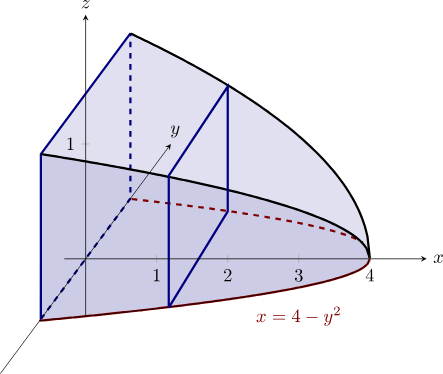
\includegraphics[width=\textwidth]{figures/accumulated_cross_sections_1.png}
    \end{minipage}
    \vspace{1em}
    \begin{minipage}{0.45\textwidth}
        \centering
        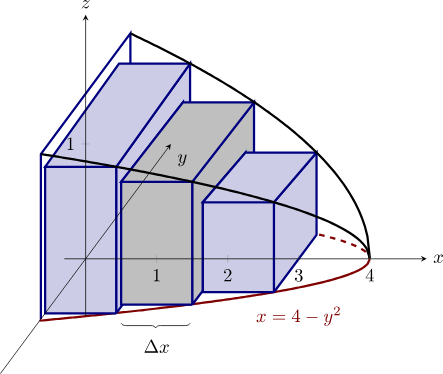
\includegraphics[width=\textwidth]{figures/accumulated_cross_sections_2.png}
    \end{minipage}
    \label{fig:volume-cross-section}
    \caption{Thể tích của khối qua diện tích mặt cắt\footnotemark}
\end{figure}
\footnotetext{nguồn \href{https://ximera.osu.edu/csccmathematics/calculus2/accumulatedCrossSections/digInAccumulatedCrossSections}{XIMERA}}

Định nghĩa này nói rằng thể tích của khối bằng ``tổng'' của diện tích tất cả các mặt cắt song song. Phương pháp này còn được gọi là \textbf{phương pháp cắt lớp}.

\begin{example}
    Thể tích của một quả cầu bán kính $R$ là $V = \dfrac{4}{3}\pi R^3$.
\end{example}
\begin{solution}
    Xét một quả cầu có tâm tại gốc tọa độ $O$ và bán kính $R$. Một lát cắt vuông góc với trục $Ox$ tại vị trí $x$ là một hình tròn. Bán kính $r$ của hình tròn này thỏa mãn $r^2 + x^2 = R^2$, suy ra $r = \sqrt{R^2 - x^2}$.
    Diện tích của mặt cắt này là:
    \[ A(x) = \pi r^2 = \pi (\sqrt{R^2 - x^2})^2 = \pi(R^2 - x^2). \]
    Do đó, thể tích của quả cầu được tính bằng cách lấy tích phân của $A(x)$ từ $-R$ đến $R$:
    \begin{align*}
        V &= \int_{-R}^R \pi(R^2 - x^2) \dd x \\
        &= \pi \left[ R^2x - \dfrac{x^3}{3} \right]_{-R}^R \\
        &= \pi \left[ \left(R^3 - \dfrac{R^3}{3}\right) - \left(-R^3 - \dfrac{(-R)^3}{3}\right) \right] \\
        &= \pi \left[ \dfrac{2R^3}{3} - \left(-\dfrac{2R^3}{3}\right) \right] = \dfrac{4}{3}\pi R^3.
    \end{align*}
\end{solution}

\begin{example}
    Một \textbf{khối tròn xoay} được tạo ra khi quay một miền phẳng quanh một đường thẳng. Giả sử $f(x) \ge 0$ trên $[a, b]$, xét khối tròn xoay thu được khi quay miền giới hạn bởi đồ thị của $f$, trục $Ox$, và hai đường thẳng $x=a, x=b$ quanh trục $Ox$. Mỗi lát cắt vuông góc tại $x$ của khối này là một hình tròn có bán kính là $f(x)$. Do đó, diện tích mặt cắt là $A(x) = \pi [f(x)]^2$. Thể tích của khối tròn xoay này là:
    \[ V = \pi \int_a^b [f(x)]^2 \dd x. \]
\end{example}

%% Ghi chú: Ví dụ gốc (5.4.5) đã được thay đổi để tránh sao chép.
\begin{example}
    Khi xoay miền giới hạn bởi đường $y = \sqrt{x}$ và trục $Ox$ trên đoạn $[0, 4]$ quanh trục $Ox$, ta được một vật thể có hình dạng paraboloid. Thể tích của khối này là:
    \[ V = \pi \int_0^4 (\sqrt{x})^2 \dd x = \pi \int_0^4 x \dd x = \pi \left[\dfrac{x^2}{2}\right]_0^4 = 8\pi. \]
\end{example}

Đề tài về diện tích và thể tích sẽ được khảo sát một cách hệ thống và tổng quát hơn trong môn Vi tích phân 2 [Bmgt2, Chương 2].

\subsection{Giá trị trung bình}

Nếu tại các điểm rời rạc $x_1, x_2, \dots, x_n$ ta có các giá trị tương ứng $f(x_1), f(x_2), \dots, f(x_n)$, thì giá trị trung bình của các giá trị này được tính bằng công thức $\dfrac{1}{n}\sum_{i=1}^n f(x_i)$. Trong trường hợp miền xác định là một khoảng liên tục $[a, b]$, ta mở rộng khái niệm này bằng cách thay phép lấy tổng bằng phép lấy tích phân.

\begin{definition}
    \textbf{Giá trị trung bình} của một hàm số $f$ khả tích trên đoạn $[a, b]$ được định nghĩa là:
    \begin{importantbox}
        \[ f_{\text{tb}} = \dfrac{1}{b-a} \int_a^b f(x) \dd x. \]
    \end{importantbox}
\end{definition}

Giá trị trung bình của một hàm số trên một miền xác định có thể được hiểu là ``tổng'' các giá trị của hàm chia cho ``độ dài'' của miền đó.

Ta có thể giải thích chi tiết hơn như sau. Chia đoạn $[a, b]$ thành $n$ đoạn con có cùng chiều dài $\Delta x = \dfrac{b-a}{n}$, với các điểm chia $a = x_0, x_1, \dots, x_n = b$. Lấy các điểm mẫu $x_i^* \in [x_{i-1}, x_i]$. Giá trị trung bình của hàm tại các điểm mẫu này là:
\[ \dfrac{f(x_1^*) + f(x_2^*) + \dots + f(x_n^*)}{n}. \]
Ta biến đổi biểu thức này:
\begin{align*}
    \dfrac{1}{n} \sum_{i=1}^n f(x_i^*) &= \dfrac{1}{b-a} \cdot \dfrac{b-a}{n} \sum_{i=1}^n f(x_i^*) \\
    &= \dfrac{1}{b-a} \sum_{i=1}^n f(x_i^*) \Delta x.
\end{align*}
Số hạng $\sum_{i=1}^n f(x_i^*) \Delta x$ chính là một tổng Riemann của $f$. Khi cho $n \to \infty$, tổng Riemann này tiến tới tích phân $\int_a^b f(x) \dd x$. Do đó, ta đi đến định nghĩa về giá trị trung bình của hàm số.

%% Ghi chú: Ví dụ gốc 5.4.6 đã được thay đổi. Mô hình nhiệt độ được thay bằng mô hình mực nước thủy triều.
%% Các hằng số và hàm lượng giác đã được điều chỉnh.
\begin{example}
    Mực nước (tính bằng mét) tại một bến cảng trong một ngày được mô hình hóa bởi hàm số $L(t) = 5 + 2\cos\left(\dfrac{\pi t}{6}\right)$, trong đó $t$ là số giờ tính từ 6 giờ sáng. Hãy tìm mực nước trung bình từ 6 giờ sáng đến 12 giờ trưa.
\end{example}
\begin{solution}
    Khoảng thời gian từ 6 giờ sáng đến 12 giờ trưa tương ứng với $t$ từ $0$ đến $6$. Giá trị trung bình của $L(t)$ trên đoạn $[0, 6]$ là:
    \begin{align*}
        L_{\text{tb}} &= \dfrac{1}{6-0} \int_0^6 \left(5 + 2\cos\left(\dfrac{\pi t}{6}\right)\right) \dd t \\
        &= \dfrac{1}{6} \left[ 5t + 2 \cdot \dfrac{6}{\pi}\sin\left(\dfrac{\pi t}{6}\right) \right]_0^6 \\
        &= \dfrac{1}{6} \left[ \left(30 + \dfrac{12}{\pi}\sin(\pi)\right) - \left(0 + \dfrac{12}{\pi}\sin(0)\right) \right] \\
        &= \dfrac{1}{6} [30] = 5.
    \end{align*}
    Vậy, mực nước trung bình trong khoảng thời gian đó là 5 mét.
\end{solution}

%% Ghi chú: Ví dụ gốc 5.4.7 là một khái niệm cơ bản nên được giữ lại, nhưng được diễn giải lại để đảm bảo tính độc đáo.
\begin{example}[Vận tốc trung bình]
    Xét một vật di chuyển trên một đường thẳng. Vị trí của vật tại thời điểm $t$ được cho bởi hàm số $x(t)$. Vận tốc tức thời $v(t)$ là đạo hàm của vị trí theo thời gian, tức là $v(t) = x'(t)$. Chú ý rằng \textbf{vận tốc (velocity)} có thể mang giá trị âm (chuyển động theo chiều ngược lại), khác với \textbf{tốc độ (speed)} là độ lớn của vận tốc và luôn không âm.
    
    Giả sử vật di chuyển trong khoảng thời gian từ $a$ đến $b$. Giá trị trung bình của vận tốc trong khoảng thời gian này là:
    \[ v_{\text{tb}} = \dfrac{1}{b-a} \int_a^b v(t) \dd t = \dfrac{1}{b-a} \int_a^b x'(t) \dd t. \]
    Theo Công thức Newton-Leibniz, ta có:
    \[ v_{\text{tb}} = \dfrac{1}{b-a} \left[ x(t) \right]_a^b = \dfrac{x(b) - x(a)}{b-a}. \]
    Kết quả này chính là định nghĩa quen thuộc của vận tốc trung bình: độ dời chia cho khoảng thời gian. Cần lưu ý rằng, vận tốc trung bình có thể khác với tốc độ trung bình (là tổng quãng đường đi được chia cho khoảng thời gian), đặc biệt là khi vật đổi chiều chuyển động.
\end{example}

\subsection{Một số ứng dụng trong khoa học}
Một trong những ý nghĩa chính của tích phân là phép tính tổng, vì vậy mỗi khi trong khoa học kỹ thuật có nhu cầu tính tổng của vô hạn các giá trị thì tích phân có thể xuất hiện. Ở đây, ta sẽ nghiên cứu các ứng dụng chủ yếu qua các ví dụ và bài toán. Người đọc có thể tham khảo thêm nhiều ví dụ ứng dụng khác trong các tài liệu như [Ste16]. TODO

\begin{example}[Mạch máu]
    Luật Poiseuille mô tả tốc độ của dòng máu chảy trong một mạch máu có dạng hình trụ:
    \[ v(r) = \dfrac{P}{4\eta l}(R^2 - r^2) \]
    trong đó $v$ là vận tốc dòng máu tại khoảng cách $r$ tính từ trục tâm, $R$ là bán kính của mạch máu, $l$ là độ dài mạch máu, $P$ là chênh lệch áp suất giữa hai đầu mạch máu, và $\eta$ là độ nhớt của máu. Ta muốn tính tổng lưu lượng máu (thể tích máu chảy qua một mặt cắt của mạch máu trong một đơn vị thời gian).
    
    Thể tích máu chảy qua một vòng xuyến mỏng có bán kính $r$ và độ dày $\dd r$ trong một đơn vị thời gian xấp xỉ bằng $v(r) \times (\text{diện tích vòng xuyến}) \approx v(r) \cdot 2\pi r \dd r$.
    Tổng lưu lượng máu trong toàn bộ mạch máu là tích phân của đại lượng này theo bán kính từ $0$ đến $R$:
    \begin{align*}
        Q = \int_0^R v(r) 2\pi r \dd r &= \int_0^R \dfrac{P}{4\eta l}(R^2 - r^2) 2\pi r \dd r \\
        &= \dfrac{2\pi P}{4\eta l} \int_0^R (R^2r - r^3) \dd r \\
        &= \dfrac{\pi P}{2\eta l} \left[ R^2\dfrac{r^2}{2} - \dfrac{r^4}{4} \right]_0^R \\
        &= \dfrac{\pi P}{2\eta l} \left( \dfrac{R^4}{2} - \dfrac{R^4}{4} \right) = \dfrac{\pi P R^4}{8\eta l}.
    \end{align*}
\end{example}

\begin{example}[Thủy lực]
    Một cửa cống hình chữ nhật, thẳng đứng, có chiều cao 15 mét và chiều rộng 40 mét. Tính tổng lực (áp lực) của nước tác động lên cửa cống nếu mực nước cao 10 mét.
\end{example}
\begin{solution}
    Áp lực của một chất lỏng tĩnh có mật độ khối lượng $\rho$ ở độ sâu $d$ được cho bởi công thức $P = \rho g d$, trong đó $g$ là gia tốc trọng trường. Nguyên lý Pascal cho biết áp lực tại một điểm trong chất lỏng tĩnh là như nhau theo mọi hướng.
    
    Ta đặt một hệ tọa độ lên mặt phẳng của cửa cống, với gốc tọa độ ở đáy cống, trục $y$ hướng thẳng đứng lên trên. Mực nước ở độ cao $y=10$.
        
    \begin{figure}[H]
        \centering
        \begin{tikzpicture}
            % Dam
            \draw[fill=gray!30] (0,0) rectangle (6,15/2.5);
            % Water
            \draw[fill=blue!20] (0,0) rectangle (6,10/2.5);
            \node at (3,12/2.5) [above] {Mực nước};
            
            % Coordinate system
            \draw[->] (-1,0) -- (7,0) node[below] {$x (m)$};
            \draw[->] (0,-1) -- (0,7) node[left] {$y (m)$};
            \node at (6,0) [below] {40};
            \node at (0,15/2.5) [left] {15};
            \node at (0,10/2.5) [left] {10};
            
            % A thin strip
            \draw[dashed, red] (0, 5/2.5) -- (6, 5/2.5);
            \node at (-0.5, 5/2.5) {$y$};
            \draw[<->] (6.2, 5/2.5) -- (6.2, 10/2.5);
            \node at (7, 7.5/2.5) {$10-y$};
        \end{tikzpicture}
        \caption{Sơ đồ tính áp lực nước lên cửa cống.}
    \end{figure}
    
    Xét một dải mỏng nằm ngang của cửa cống ở độ cao $y$ với độ dày $\dd y$. Độ sâu của dải này là $10-y$. Áp lực nước tại độ sâu này là $P(y) = \rho g (10-y)$.
    Diện tích của dải mỏng là $dA = 40 \dd y$. Lực tác động lên dải này là $\dd F = P(y) \dd A = \rho g (10-y) (40 \dd y)$.
    Tổng lực tác động lên toàn bộ phần ngập nước của cửa cống là tích phân của $\dd F$ từ $y=0$ đến $y=10$. Với $\rho_{\text{nước}} \approx 1000$ kg/m$^3$ và $g \approx 9,8$ m/s$^2$:
    \begin{align*}
        F = \int_0^{10} 40 \rho g (10-y) \dd y &= 40 \cdot 1000 \cdot 9,8 \int_0^{10} (10-y) \dd y \\
        &= 392000 \left[ 10y - \dfrac{y^2}{2} \right]_0^{10} \\
        &= 392000 \left( 100 - \dfrac{100}{2} \right) \\
        &= 392000 \cdot 50 = 19,6 \cdot 10^6 \text{ (N)}.
    \end{align*}
    Đơn vị của lực là Newton (N).
\end{solution}

\subsubsection{Hàm mật độ}
Nếu tại mỗi điểm $x_i$ ($1 \le i \le n$) có một đại lượng tương ứng là $f(x_i)$, thì tổng giá trị của đại lượng đó là $\sum_{i=1}^n f(x_i)$. Khi tập hợp các điểm $D$ là một khoảng liên tục, hàm $f$ từ $D$ vào $\R$ được gọi là \textbf{hàm mật độ} của đại lượng, và tổng giá trị của đại lượng là tích phân $\int_D f(x) \dd x$.
Trong vật lý, khối lượng của một vật là tích phân của hàm mật độ khối lượng trên miền không gian mà vật chiếm giữ.

\begin{example}
    Tìm khối lượng của một sợi dây dài 1 mét có mật độ khối lượng tuyến tính (khối lượng trên một đơn vị chiều dài) là $\rho(x) = 1 + \sin(\pi x)$ (kg/m), với $x$ là khoảng cách từ một đầu của sợi dây.
\end{example}
\begin{solution}
    Khối lượng của sợi dây bằng tích phân của hàm mật độ khối lượng trên suốt chiều dài của nó:
    \begin{align*}
        M = \int_0^1 \rho(x) \dd x &= \int_0^1 (1 + \sin(\pi x)) \dd x \\
        &= \left[ x - \dfrac{1}{\pi}\cos(\pi x) \right]_0^1 \\
        &= \left( 1 - \dfrac{1}{\pi}\cos(\pi) \right) - \left( 0 - \dfrac{1}{\pi}\cos(0) \right) \\
        &= \left( 1 + \dfrac{1}{\pi} \right) - \left( -\dfrac{1}{\pi} \right) = 1 + \dfrac{2}{\pi} \approx 1,637 \text{ (kg)}.
    \end{align*}
\end{solution}

\subsubsection{Công}
Giả sử một vật di chuyển dưới tác dụng của một lực. \textbf{Công} của lực là một khái niệm vật lý đại diện cho năng lượng mà lực truyền cho vật trong quá trình di chuyển.
Nếu một vật di chuyển một quãng đường $d$ trên một đường thẳng dưới tác dụng của một lực không đổi $F$ cùng chiều chuyển động, công sinh ra được định nghĩa là $W = F \cdot d$.

Bây giờ, xét trường hợp tổng quát hơn, khi lực $F$ có thể thay đổi độ lớn theo vị trí, nhưng vẫn cùng phương với chuyển động. Đặt một trục tọa độ dọc theo phương chuyển động. Độ lớn của lực tác dụng lên vật tại vị trí $x$ là $F(x)$. Giả sử vật di chuyển từ vị trí $x=a$ đến vị trí $x=b$. Công của lực $F$ là ``tổng'' của các giá trị $F(x)$ trên suốt quãng đường, được cho bởi tích phân:
\[ W = \int_a^b F(x) \dd x. \]

\begin{example}[Định lý công-động năng]
    Giả sử một vật có khối lượng $m$ di chuyển dưới tác dụng của một tổng hợp lực $F$. Vị trí của vật tại thời điểm $t$ là $x(t)$, vận tốc là $v(t) = x'(t)$, và gia tốc là $a(t) = v'(t) = x''(t)$. Giả sử vật di chuyển từ $x(t_0) = a$ đến $x(t_1) = b$. \textbf{Động năng} (năng lượng do chuyển động) của vật là $K(t) = \dfrac{1}{2}mv(t)^2 = \dfrac{1}{2}m[x'(t)]^2$.
    
    Theo định luật II Newton: $F = ma = mx''$. Do đó, công của lực $F$ khi vật di chuyển từ $a$ đến $b$ là:
    \[ W = \int_a^b F(x) \dd x = \int_{t_0}^{t_1} F(x(t)) x'(t) \dd t = \int_{t_0}^{t_1} m x''(t) x'(t) \dd t. \]
    Sử dụng hằng đẳng thức $\deriv{}{t} [x'(t)]^2 = 2x'(t)x''(t)$, ta biến đổi:
    \begin{align*}
        W = \int_{t_0}^{t_1} m \cdot \dfrac{1}{2} \deriv{}{t}[x'(t)]^2 \dd t &= \dfrac{1}{2}m \int_{t_0}^{t_1} \deriv{}{t}[x'(t)]^2 \dd t \\
        &= \dfrac{1}{2}m [x'(t)]^2 \bigg|_{t_0}^{t_1} \\
        &= \dfrac{1}{2}m[x'(t_1)]^2 - \dfrac{1}{2}m[x'(t_0)]^2 = K(t_1) - K(t_0).
    \end{align*}
    Vậy, ta thu được bằng phương pháp toán học một định luật vật lý quan trọng: \textbf{công của ngoại lực tác dụng lên vật bằng độ biến thiên động năng của vật đó}.
\end{example}

\subsection{Xác suất}

Trong lý thuyết xác suất, một \textbf{biến ngẫu nhiên} $X$ là một ánh xạ từ một tập hợp các sự kiện vào tập hợp các số thực.

\subsubsection{Biến ngẫu nhiên rời rạc}
Trong trường hợp tập giá trị $D$ của $X$ là hữu hạn, ta nói $X$ là một \textbf{biến ngẫu nhiên rời rạc}. Với mỗi giá trị $x \in D$, có một số thực $0 \le p(x) \le 1$ là xác suất để $X$ có giá trị $x$ (giá trị 1 tương ứng với 100\%). Hàm $p$ được gọi là \textbf{hàm xác suất} của biến ngẫu nhiên $X$. Xác suất để $X$ có giá trị nằm trong một tập con $C \subset D$ được cho bởi:
\[ P(X \in C) = \sum_{x \in C} p(x). \]
Một hệ quả là tổng xác suất trên toàn bộ không gian mẫu phải bằng 1, tức là $\sum_{x \in D} p(x) = 1$. \textbf{Giá trị trung bình} (mean) hay \textbf{kỳ vọng} (expectation) của $X$ được cho bởi:
\[ E[X] = \sum_{x \in D} x \cdot p(x). \]

\begin{example}
    Xét một trò chơi tung đồng xu công bằng như sau: Người chơi trả 5 nghìn đồng cho mỗi lần tung. Nếu mặt ngửa xuất hiện, người chơi nhận được 8 nghìn đồng. Nếu mặt sấp xuất hiện, người chơi không nhận được gì. Hỏi trung bình người chơi sẽ lãi hay lỗ?
\end{example}
\begin{solution}
    Gọi $X$ là số tiền người chơi nhận được. $X$ có thể nhận hai giá trị: $8$ (nếu ngửa) và $0$ (nếu sấp). Vì đồng xu công bằng, xác suất của mỗi kết quả là $1/2$.
    Hàm xác suất là $p(8) = 1/2$ và $p(0) = 1/2$.
    Kỳ vọng của số tiền nhận được là:
    \[ E[X] = 8 \cdot p(8) + 0 \cdot p(0) = 8 \cdot \dfrac{1}{2} + 0 \cdot \dfrac{1}{2} = 4. \]
    Kỳ vọng số tiền nhận được là 4 nghìn đồng, trong khi chi phí mỗi lần chơi là 5 nghìn đồng. Như vậy, về lâu dài, trung bình mỗi lần chơi người chơi sẽ lỗ 1 nghìn đồng.
\end{solution}

\subsubsection{Biến ngẫu nhiên liên tục}
Trong trường hợp tập giá trị của biến ngẫu nhiên $X$ là một khoảng số thực $D$ (có thể là $(-\infty, \infty)$), ta nói $X$ là một \textbf{biến ngẫu nhiên liên tục}. Tương tự với trường hợp rời rạc, có một \textbf{hàm mật độ xác suất} (probability density function - PDF) $f$ xác định trên $D$ sao cho $f(x) \ge 0$ và xác suất để $X$ có giá trị trong một khoảng $[c, d] \subset D$ được tính bằng tích phân:
\[ P(c \le X \le d) = \int_c^d f(x) \dd x. \]
Hàm mật độ xác suất phải thỏa mãn điều kiện chuẩn hóa:
\[ \int_D f(x) \dd x = 1. \]
Tương tự, kỳ vọng của biến ngẫu nhiên liên tục $X$ được tính bằng tích phân:
\[ E[X] = \int_D x f(x) \dd x. \]

%% Ghi chú: Ví dụ gốc 5.4.13 đã được thay đổi. Mô hình tuổi thọ của bóng đèn được sử dụng thay cho sản phẩm.
\begin{example}
    Gọi $T$ là biến ngẫu nhiên biểu thị tuổi thọ của một loại bóng đèn LED (tính bằng nghìn giờ). Giả sử hàm mật độ xác suất của $T$ là $f(t) = 0.05e^{-0.05t}$ với $t \ge 0$.
\end{example}
\begin{solution}
    (a) Xác suất một bóng đèn hỏng trong vòng 10,000 giờ đầu tiên (tức là $0 \le T \le 10$) là:
    \[ P(0 \le T \le 10) = \int_0^{10} 0.05e^{-0.05t} \dd t = \left[-e^{-0.05t}\right]_0^{10} = -e^{-0.5} - (-e^0) = 1 - e^{-0.5} \approx 0.393. \]
    Vậy có khoảng 39.3\% khả năng bóng đèn sẽ hỏng trong 10,000 giờ đầu.

    (b) Tuổi thọ trung bình (kỳ vọng) của bóng đèn là:
    \[ E[T] = \int_0^\infty t \cdot f(t) \dd t = \int_0^\infty 0.05t e^{-0.05t} \dd t. \]
    Ta tính tích phân từng phần với $u = t$ và $\dd v = 0.05e^{-0.05t} \dd t$. Suy ra $\dd u = \dd t$ và $v = -e^{-0.05t}$.
    \begin{align*}
        E[T] &= \lim_{h \to \infty} \left( [-te^{-0.05t}]_0^h - \int_0^h (-e^{-0.05t}) \dd t \right) \\
        &= \lim_{h \to \infty} \left( -he^{-0.05h} - \left[ \dfrac{1}{0.05}e^{-0.05t} \right]_0^h \right) \\
        &= \lim_{h \to \infty} \left( -he^{-0.05h} - 20(e^{-0.05h} - 1) \right).
    \end{align*}
    Sử dụng quy tắc L'Hôpital, $\lim_{h \to \infty} he^{-0.05h} = \lim_{h \to \infty} \frac{h}{e^{0.05h}} = 0$.
    Do đó, $E[T] = 0 - 20(0 - 1) = 20$.
    Vậy, tuổi thọ trung bình của bóng đèn là 20,000 giờ.
\end{solution}

\begin{example}[Phân bố chuẩn]
    Nhiều hiện tượng ngẫu nhiên trong tự nhiên và xã hội được mô hình hóa bằng \textbf{phân bố chuẩn} (normal distribution), với hàm mật độ xác suất có dạng:
    \[ f(x) = \dfrac{1}{\sigma\sqrt{2\pi}} e^{-\frac{(x-\mu)^2}{2\sigma^2}}. \]
    Ở đây, $\mu$ là giá trị trung bình (kỳ vọng) và $\sigma$ là \textbf{độ lệch chuẩn} (standard deviation), đo lường mức độ phân tán của các giá trị. Đồ thị của hàm này có dạng hình chuông đặc trưng.
        Việc đây thực sự là một hàm mật độ xác suất là hệ quả của một công thức tích phân nổi tiếng:
    \[ \int_{-\infty}^\infty e^{-x^2} \dd x = \sqrt{\pi}. \]
    Công thức quan trọng này có thể được chứng minh bằng cách sử dụng tích phân của hàm hai biến trong [Bmgt2, Chương 2].
    
    Môn học Xác suất Thống kê sẽ thảo luận chi tiết hơn về chủ đề này ([NTNM22], [Ros20]).
\end{example}

\subsection{Bài tập}
\subsubsection{Diện tích, thể tích}

\begin{exercise}
    Tính diện tích của miền được giới hạn bởi các đường cong đã cho.
    \begin{enumerate}[label=(\alph*)]
        \item $y = x^2 - 2x$ và $y = x+4$.
        \item $y = x^3 - x$ và $y = 3x$.
        \item $y = \sin x$, $y = \cos x$, $x=0$, và $x=\pi/2$.
        \item $y = (x-2)^2$ và $y=x$.
        \item $y = |x|$ và $y = x^2 - 2$.
        \item $x = 2y^2$ và $x = 4+y^2$.
        \item $y = 1/x$, $y=x^2$, $y=0$, $x=e$.
        \item $y = e^x$, $y=e^{-x}$, và $x=1$.
        \item $y = x^4 - 4x^2 + 4$ và $y=x^2$.
        \item $y=x\sqrt{x-1}$ và $y=2\sqrt{x-1}$.
        \item $x=y^3-y$ và $x=0$.
        \item $y = \dfrac{1}{1+x^2}$ và $y = \dfrac{1}{2}|x|$.
    \end{enumerate}
\end{exercise}

\begin{exercise}
    Sử dụng chương trình máy tính (tham khảo Hướng dẫn ở trang 187) để vẽ đồ thị và tìm diện tích (xấp xỉ) của miền được giới hạn bởi các đường cong:
    \begin{enumerate}[label=(\alph*)]
        \item $y = x^5 - 6x^3 + 4x$ và $y=x$.
        \item $y = x \cos(x^2)$ và $y = x^3 - x$.
    \end{enumerate}
\end{exercise}

\begin{exercise}
    Một máy chụp cắt lớp vi tính (CAT scan) tạo ra các hình ảnh cắt ngang của một cơ quan trong cơ thể. Giả sử máy quét chụp các lát cắt của một lá gan, với các lát cắt cách đều nhau 1 cm. Cho biết chiều dài của lá gan là 10 cm và diện tích của các mặt cắt ngang (đơn vị cm$^2$) tại các vị trí $x=0, 1, ..., 10$ lần lượt là: 0, 25, 60, 85, 105, 110, 100, 80, 50, 15, 0. Hãy dùng tổng Riemann (ví dụ: quy tắc hình thang hoặc quy tắc trung điểm) để ước tính thể tích của lá gan.
\end{exercise}

\begin{exercise}
    Tìm thể tích của khối tròn xoay được tạo thành khi quay miền được giới hạn bởi các đường cong cho trước quanh trục đã chỉ định, Hình~\ref{fig:volumn_solid_revolution}.
    
    % Placeholder for the image of the solid of revolution
    \begin{figure}[H]
        \centering
        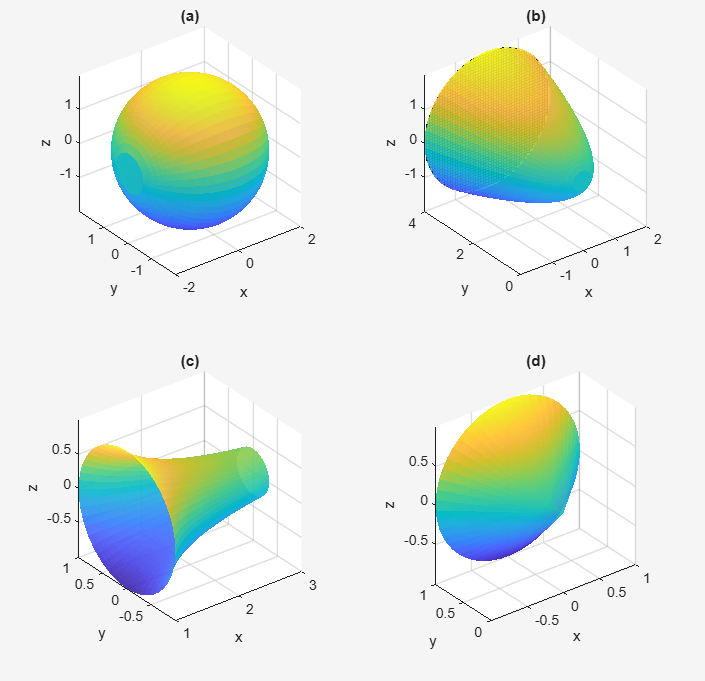
\includegraphics[width=0.8\linewidth]{figures/volumn_solid_revolution.png}
        \caption{Thể tích của các khối tạo bởi đường cong quay quanh trục}
        \label{fig:volumn_solid_revolution}
    \end{figure}
    
    \begin{enumerate}[label=(\alph*)]
        \item $y = \sqrt{4-x^2}$, $y=0$, quanh trục $x$.
        \item $y = x^2$, $y=4$, $x=0$, quanh trục $y$.
        \item $y = 1/x$, $x=1$, $x=3$, $y=0$, quanh trục $x$.
        \item $y = x$, $y = \sqrt{x}$, quanh trục $y$.
    \end{enumerate}
\end{exercise}

\begin{exercise}
    Tìm thể tích của khối được tạo bằng cách xoay miền bao bởi đồ thị của hàm số $f(x) = x(x-1)^2$ và trục $x$ quanh trục $y$.
\end{exercise}

\begin{exercise}
    Chứng tỏ rằng ``sừng Gabriel'', là khối không gian nhận được bằng cách xoay quanh trục $x$ phần mặt phẳng bên dưới đồ thị của hàm $y = 1/x$ bên trên trục $x$ với $x \ge 1$, có thể tích hữu hạn nhưng diện tích bề mặt là vô hạn.
\end{exercise}

\begin{exercise}
    Tính thể tích của các khối rắn $S$ được mô tả sau đây.
    \begin{enumerate}[label=(\alph*)]
        \item Một khối nón thẳng đứng có chiều cao $h$ và bán kính đáy $r$.
        \item Một khối chóp cụt có chiều cao $h$, đáy dưới là hình vuông cạnh $B$, và đáy trên là hình vuông cạnh $b$.
        \item Một nắp chỏm cầu có chiều cao $h$ được cắt từ một quả cầu có bán kính $r$.
        \item Một khối chóp có chiều cao $h$ và đáy là một tam giác đều cạnh $a$.
        \item Một khối chóp có chiều cao $h$ và đáy là một hình chữ nhật có kích thước $L \times W$.
        \item Một cái nêm được cắt ra từ một khối trụ (bán kính 5) bởi một mặt phẳng đi qua đường kính của đáy và một mặt phẳng khác nghiêng một góc 45 độ so với đáy.
        \item Một khối có đáy là hình tròn $x^2+y^2=4$. Các mặt cắt vuông góc với trục $x$ là các tam giác vuông cân có cạnh góc vuông nằm trên đáy.
    \end{enumerate}
\end{exercise}

\begin{exercise}
    Một bể chứa nước có dạng hình nón ngược với chiều cao 10m và bán kính đáy 4m. Bể đang chứa nước đến độ cao 8m. Tính công cần thiết để bơm toàn bộ nước ra khỏi miệng bể. (Khối lượng riêng của nước là $\rho = 1000$ kg/m$^3$).
\end{exercise}

\begin{exercise}
    Một quả bóng bay hình cầu đang được bơm không khí vào. Khi bán kính của nó đạt 15 cm, thể tích của quả cầu đang tăng với tốc độ 100 cm$^3$/s. Hỏi lúc đó bán kính của quả cầu đang tăng với tốc độ bao nhiêu?
\end{exercise}

\begin{exercise}
    Tìm thể tích của một ``cái đĩa'' (torus) được tạo ra bằng cách quay một hình tròn bán kính $r$ quanh một trục nằm trong mặt phẳng của hình tròn và cách tâm hình tròn một khoảng $R$ (với $R > r$).

    \begin{figure}
        \centering
        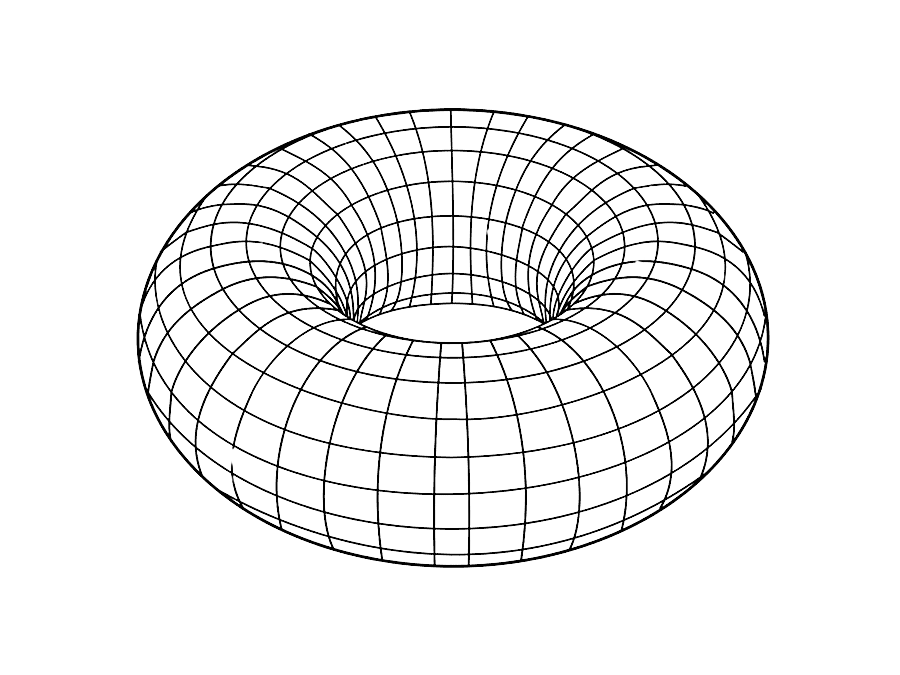
\includegraphics[width=0.6\linewidth]{figures/torus.png}
        \caption{Minh hoa cho hình Torus}
        \label{fig:torus}
    \end{figure}
    
\end{exercise}

\begin{exercise}
    Một bể bơi có hình dạng và kích thước như trong hình vẽ (đơn vị là mét). Bể bơi dài 20m, rộng 10m. Mực nước sâu 1m ở đầu cạn và 3m ở đầu sâu, với đáy dốc đều. Nếu bể chứa đầy nước, hãy tính công cần thiết để bơm hết nước ra khỏi thành bể.
\end{exercise}

\subsubsection{Ứng dụng trong vật lý}

\begin{exercise}
    Một chiếc xe đang di chuyển trên đường thẳng với vận tốc 88 ft/s thì người lái xe đạp phanh gấp. Xe giảm tốc với gia tốc không đổi là 11 ft/s$^2$.
    \begin{enumerate}[label=(\alph*)]
        \item Viết công thức cho vận tốc của xe sau $t$ giây kể từ lúc đạp phanh. Sau bao lâu thì xe dừng hẳn?
        \item Viết công thức cho quãng đường xe đi được sau $t$ giây kể từ lúc đạp phanh. Tính quãng đường xe đi được cho đến khi dừng hẳn.
    \end{enumerate}
\end{exercise}

\begin{exercise}
    Một dây cáp đồng nhất dài 10 mét và nặng 50 kg được treo thẳng đứng. Tính công cần thiết để kéo toàn bộ dây cáp lên đỉnh.
\end{exercise}

\begin{exercise}
    Một bể chứa nước hình bán cầu với bán kính 5 mét đang chứa đầy nước. Tính công cần thiết để bơm toàn bộ nước ra khỏi miệng bể. (Khối lượng riêng của nước là $\rho = 1000$ kg/m$^3$).
\end{exercise}

\begin{exercise}
    Theo định luật vạn vật hấp dẫn của Newton, lực hấp dẫn giữa hai vật có khối lượng $m_1$ và $m_2$ là $F = G \frac{m_1 m_2}{r^2}$, trong đó $r$ là khoảng cách giữa hai vật và $G$ là hằng số hấp dẫn.
    \begin{enumerate}[label=(\alph*)]
        \item Giả sử một trong hai vật được giữ cố định. Tính công cần thiết để di chuyển vật còn lại từ vị trí $r=a$ đến $r=b$.
        \item Tính công (năng lượng) cần thiết để phóng một tàu vũ trụ nặng 2000 kg từ bề mặt Trái Đất ra khỏi trường hấp dẫn của nó (tức là đến vô cùng).
    \end{enumerate}
    Giả sử khối lượng Trái Đất là $5.98 \times 10^{24}$ kg, bán kính Trái Đất là $6.37 \times 10^6$ m, và $G = 6.67 \times 10^{-11}$ N$\cdot$m$^2$/kg$^2$.
\end{exercise}

\begin{exercise}
    Dòng điện xoay chiều trong một mạch điện gia dụng có điện thế thay đổi theo phương trình $E(t) = A \sin(\omega t)$, trong đó $A$ là biên độ điện thế, $\omega$ là tần số góc. Các vôn kế đo \textbf{điện thế hiệu dụng} ($V_{rms}$), được định nghĩa là căn bậc hai của giá trị trung bình của $[E(t)]^2$ trong một chu kỳ.
    \[ V_{rms} = \sqrt{\frac{1}{T} \int_0^T [E(t)]^2 \dd t}. \]
    \begin{enumerate}[label=(\alph*)]
        \item Chứng minh rằng $V_{rms} = \frac{A}{\sqrt{2}}$.
        \item Một dòng điện gia dụng ở Việt Nam có điện thế hiệu dụng là 220V. Tìm biên độ điện thế $A$ của dòng điện này.
    \end{enumerate}
\end{exercise}

\begin{exercise}
    Một lò xo tuân theo định luật Hooke, tức là lực cần thiết để giữ lò xo bị kéo dãn một đoạn $x$ so với vị trí cân bằng là $F = kx$, trong đó $k$ là hằng số lò xo.
    \begin{enumerate}[label=(\alph*)]
        \item Nếu cần một lực 40 N để giữ một lò xo bị kéo dãn 10 cm, hãy tính công cần thiết để kéo dãn lò xo từ vị trí cân bằng đến 15 cm.
        \item Tính công cần thiết để kéo dãn lò xo thêm 5 cm nữa (từ 15 cm đến 20 cm).
    \end{enumerate}
\end{exercise}

\subsubsection{Ứng dụng trong kinh tế}

\begin{exercise}
    Hàm chi phí biên (marginal cost) để sản xuất $x$ đơn vị sản phẩm được cho bởi $C'(x) = 0.003x^2 - 0.8x + 75$. Chi phí cố định là $C(0) = 4000$.
    \begin{enumerate}[label=(\alph*)]
        \item Tìm hàm chi phí $C(x)$.
        \item Tính chi phí trung bình để sản xuất từ 100 đến 200 đơn vị sản phẩm.
    \end{enumerate}
\end{exercise}

\begin{exercise}
    Hàm doanh thu biên (marginal revenue) từ việc bán $q$ sản phẩm là $R'(q) = 450 - 0.8q$. Biết rằng không có doanh thu khi không có sản phẩm nào được bán.
    \begin{enumerate}[label=(\alph*)]
        \item Tìm hàm doanh thu $R(q)$.
        \item Tìm hàm cầu (demand function) $p(q)$, là giá bán của mỗi sản phẩm.
    \end{enumerate}
\end{exercise}

\begin{exercise}
    Hàm cung ứng (supply function) cho một sản phẩm là $p = S(x) = 10 + 0.1x + 0.0005x^2$, trong đó $p$ là giá bán mỗi đơn vị và $x$ là số lượng sản phẩm được cung ứng.
    \begin{enumerate}[label=(\alph*)]
        \item Tìm giá trung bình của sản phẩm khi mức cung ứng nằm trong khoảng từ 0 đến 50 đơn vị.
        \item Tìm mức cung ứng $x_0$ sao cho giá trung bình trong khoảng $[0, x_0]$ bằng 20.
    \end{enumerate}
\end{exercise}

\begin{exercise}
    Một công ty sản xuất máy tính xách tay. Phương trình cầu cho sản phẩm là $p = 1200 - 1.5x$, và hàm chi phí là $C(x) = 400x + 5000$, với $0 \le x \le 500$.
    \begin{enumerate}[label=(\alph*)]
        \item Tìm hàm lợi nhuận $P(x)$.
        \item Vẽ đồ thị hàm lợi nhuận.
        \item Với quy mô sản xuất nào thì công ty bắt đầu có lãi?
        \item Tìm quy mô sản xuất để đạt lợi nhuận tối đa.
        \item Tìm lợi nhuận trung bình nếu công ty sản xuất trong khoảng từ 200 đến 300 máy.
        \item Giả sử chính phủ đánh thuế 50 đô la trên mỗi máy bán ra. Công ty nên đặt giá bán mới là bao nhiêu để tối đa hóa lợi nhuận?
    \end{enumerate}
\end{exercise}

\begin{exercise}
    Một mỏ dầu đang sản xuất dầu với tốc độ $P'(t) = 120e^{-0.05t}$, trong đó $P'(t)$ được tính bằng nghìn thùng mỗi năm, và $t$ là số năm kể từ bây giờ.
    \begin{enumerate}[label=(\alph*)]
        \item Tổng sản lượng dầu sẽ được khai thác trong 5 năm tới là bao nhiêu?
        \item Giả sử mỏ dầu sẽ cạn kiệt. Hãy ước tính tổng trữ lượng dầu của mỏ.
    \end{enumerate}
\end{exercise}

\begin{exercise}
    Dòng tiền (cash flow) của một dự án đầu tư được dự đoán là $f(t) = 2000\sqrt{t+1}$ (đô la mỗi năm) trong vòng 8 năm tới. Nếu lãi suất chiết khấu liên tục là 5\% mỗi năm, hãy tính giá trị hiện tại (present value) của dòng tiền này.
    (Gợi ý: Giá trị hiện tại của một dòng tiền $f(t)$ trong khoảng $[0, T]$ với lãi suất $r$ là $\int_0^T f(t)e^{-rt} \dd t$).
\end{exercise}

\subsubsection{Xác suất}

\begin{exercise}
    Một biến ngẫu nhiên liên tục $X$ có hàm mật độ xác suất dạng $f(x) = kx(4-x)$, với $0 \le x \le 4$ và $k$ là một hằng số.
    \begin{enumerate}[label=(\alph*)]
        \item Tìm giá trị của hằng số $k$ để $f(x)$ là một hàm mật độ xác suất.
        \item Vẽ đồ thị của hàm mật độ xác suất $f(x)$.
        \item Tìm xác suất để biến ngẫu nhiên $X$ có giá trị nằm trong khoảng $[1, 2]$.
        \item Tìm xác suất để biến ngẫu nhiên $X$ có giá trị lớn hơn 3.
        \item Tính giá trị trung bình (kỳ vọng) của biến ngẫu nhiên này.
    \end{enumerate}
\end{exercise}

\begin{exercise}
    Tuổi thọ của một loại linh kiện điện tử (tính bằng giờ) được cho bởi hàm mật độ xác suất $f(x) = 0.001e^{-0.001x}$ với $x \ge 0$.
    \begin{enumerate}[label=(\alph*)]
        \item Vẽ đồ thị của hàm mật độ xác suất.
        \item Hãy kiểm tra rằng $f(x)$ thỏa mãn yêu cầu của một hàm mật độ xác suất.
        \item Tìm xác suất để một linh kiện hoạt động được ít nhất 500 giờ.
        \item Tìm xác suất để một linh kiện hỏng trong vòng 200 giờ đầu tiên.
        \item Tính tuổi thọ trung bình của loại linh kiện này.
    \end{enumerate}
\end{exercise}

\begin{exercise}
    Giả sử chiều cao của nam giới trưởng thành tại một quốc gia tuân theo phân phối chuẩn với giá trị trung bình là 175 cm và độ lệch chuẩn là 7 cm.
    \begin{enumerate}[label=(\alph*)]
        \item Viết công thức hàm mật độ xác suất cho biến ngẫu nhiên này.
        \item Tìm xác suất để một người đàn ông được chọn ngẫu nhiên có chiều cao từ 170 cm đến 180 cm. (Sử dụng máy tính để tính tích phân).
        \item Nếu một câu lạc bộ bóng rổ chỉ tuyển những người cao trên 190 cm, hãy ước tính tỉ lệ phần trăm nam giới trưởng thành đủ điều kiện tham gia.
    \end{enumerate}
\end{exercise}

\begin{exercise}
    Thời gian chờ xe buýt tại một trạm (tính bằng phút) là một biến ngẫu nhiên phân phối đều trên khoảng $[0, 15]$. Hàm mật độ xác suất là $f(x) = 1/15$ với $0 \le x \le 15$.
    \begin{enumerate}[label=(\alph*)]
        \item Tìm xác suất để một hành khách phải chờ từ 5 đến 10 phút.
        \item Tìm xác suất để hành khách phải chờ ít hơn 3 phút.
        \item Tính thời gian chờ trung bình.
    \end{enumerate}
\end{exercise}

\subsubsection{Các bài toán khác}

\begin{exercise}
    Nhiệt độ trong một ngày ở sa mạc có thể được mô hình hóa bởi hàm số $T(t) = 35 + 15\cos\left(\frac{\pi}{12}(t-4)\right)$, trong đó $t$ là số giờ kể từ nửa đêm. Tìm nhiệt độ trung bình trong khoảng thời gian từ 6 giờ sáng ($t=6$) đến 6 giờ tối ($t=18$).
\end{exercise}

\begin{exercise}
    Nồng độ của một loại thuốc trong máu của bệnh nhân sau $t$ giờ kể từ khi tiêm được mô hình hóa bởi hàm số $C(t) = 10te^{-0.5t}$ (mg/L).
    \begin{enumerate}[label=(\alph*)]
        \item Tính nồng độ trung bình của thuốc trong máu trong 4 giờ đầu tiên.
        \item Sử dụng máy tính để vẽ đồ thị hàm nồng độ. Tại thời điểm nào nồng độ thuốc đạt cực đại?
    \end{enumerate}
\end{exercise}

\begin{exercise}
    Ta đi từ nhà đến trường, một quãng đường dài 5 km, và mất tổng cộng 15 phút (0.25 giờ). Vận tốc trung bình của cả chuyến đi là $5 / 0.25 = 20$ km/h. Hãy giải thích tại sao chắc chắn phải có một thời điểm trong chuyến đi mà vận tốc tức thời của ta đúng bằng 20 km/h. (Gợi ý: Sử dụng Định lý Giá trị Trung bình cho Tích phân hoặc Định lý Giá trị Trung bình cho Đạo hàm).
\end{exercise}

\begin{exercise}
    Số lượng người (tính bằng nghìn người) đến một công viên giải trí trong một ngày được mô hình hóa bởi tốc độ $r(t) = 2 - 2\cos\left(\frac{\pi}{6}t\right)$, trong đó $t$ là số giờ kể từ lúc công viên mở cửa lúc 8 giờ sáng ($t=0$).
    \begin{enumerate}[label=(\alph*)]
        \item Công viên mở cửa trong 12 giờ. Tính tổng số lượt khách trong ngày.
        \item Tính số lượt khách trung bình mỗi giờ trong 4 giờ đầu tiên công viên mở cửa.
    \end{enumerate}
\end{exercise}

\begin{exercise}
    Lượng người đang bị mắc một bệnh truyền nhiễm (tính bằng nghìn người) vào thời điểm $t$ (tính bằng ngày kể từ khi dịch bùng phát) được mô hình hóa bởi hàm $N(t) = 25 t^2 e^{-t/5}$, với $0 \le t \le 40$.
    \begin{enumerate}[label=(\alph*)]
        \item Vẽ đồ thị của hàm số này bằng máy tính.
        \item Tìm thời điểm mà số người đang nhiễm bệnh đạt cực đại.
        \item Khi nào thì số người đang nhiễm bệnh bắt đầu giảm?
        \item Khi nào thì tốc độ lây nhiễm bắt đầu chậm lại (tức là tìm điểm uốn của đồ thị)?
        \item Tính số lượng người bệnh trung bình trong 20 ngày đầu tiên của đợt dịch.
    \end{enumerate}
\end{exercise}

\begin{exercise}
    Một nhà sinh thái học mô hình hóa quần thể của một loài cá trong hồ bằng phương trình logistic. Tốc độ tăng trưởng của quần thể được cho bởi $\frac{dP}{dt} = 0.2P\left(1 - \frac{P}{5000}\right)$, trong đó $P(t)$ là số lượng cá tại thời điểm $t$ (tính bằng năm).
    \begin{enumerate}[label=(\alph*)]
        \item Tốc độ tăng trưởng của quần thể lớn nhất khi nào? (Gợi ý: Tìm cực đại của hàm $\frac{dP}{dt}$).
        \item Nếu $P(0) = 1000$, hãy giải phương trình vi phân này để tìm $P(t)$. (Đây là một bài toán nâng cao, có thể tham khảo thêm sách về phương trình vi phân).
    \end{enumerate}
\end{exercise}
